\section{Random variables}

\mode<presentation>{
%---------------------------------------------------------------------slide----
\begin{frame}
\frametitle{Random variables}

\tableofcontents[sectionstyle=show/hide,hideothersubsections]
\end{frame}
}


%---------------------------------------------------------------------slide----
\begin{frame}
\frametitle{Random variables}
The process of drawing a sample randomly is a random experiment and any variable measured in the sample is a
\emph{random variable} cause the values taken by the variable in the individuals of the sample is a matter of chance.

\begin{definition}[Random variable] 
A \emph{random variable} $X$ is a function that maps every element of the sample space of a random experiment to a real
number.
\[ 
X:\Omega \rightarrow \mathbb{R} 
\]

The set of values that the variable can assume is called \remph{range} and is represented $R.
\end{definition}

In essence, a random variable is a variable whose values come from a random experiment, and every value have
a probability of occurrence. 

\highlight{\textbf{Example}}. The variable $X$ that measures the outcome of rolling a dice is a random variable and its
range is 
\[
\mbox{Range}(X)=\{1,2,3,4,5,6\}
\]
\end{frame}


%---------------------------------------------------------------------slide----
\begin{frame}
\frametitle{Types of random variables}
There are two types of random variables:
\begin{description}
\item[Discrete] They take isolated values, and their range is numerable.\\
Example. Number of children of a family, number of smoked cigarettes, number of subjects passed, etc.
\item[Continuous] They can take any value in an real interval, and their range is non-numerable.\\
Example. Weight, height, age, cholesterol level, etc. 
\end{description}

The way of modelling every type of variable is different. 
In this chapter we are going to study how to model discrete variables.
\end{frame}


\subsection{Probability distribution of a discrete random variable}

%---------------------------------------------------------------------slide----
\begin{frame}
\frametitle{Probability distribution of a discrete random variable}
As values of a discrete random variable are linked to the elementary events of a random experiment, every value have a
probability. 
\begin{definition}[Probability function]
The \emph{probability function} of a discrete random variable $X$ is the function $f(x)$ that maps every value $x_i$ of
the variable to its probability
\[
f(x_i) = P(X=x_i).
\]
\end{definition}

We can also accumulate probabilities the same way that we accumulated sample frequencies. 

\begin{definition}[Distributin function]
The \emph{distribution function} of a discrete random variable $X$ is the function $F(x)$ that maps every value $x_i$ of
the variable to the probability of having a value less than or equal to $x_i$ 
\[
F(x_i) = P(X\leq x_i) = f(x_1)+\cdots +f(x_i).
\]
\end{definition}
\end{frame}


%---------------------------------------------------------------------slide----
\begin{frame}
\frametitle{Probability distribution of a discrete random variable}
The range of a discrete random variable and its probability function is known as \highlight{\textbf{Probability
Distribution}} of the variable, and usually it is presented in a table 

\[
\begin{array}{|c|cccc|c|}
\hline
X & x_1 & x_2 & \cdots & x_n & \sum\\ \hline
f(x) & f(x_1) & f(x_2) & \cdots & f(x_n) & 1\\
\hline
F(x) & F(x_1) & F(x_2) & \cdots & F(x_n) =1 &\multicolumn{1}{|c}{} \\
\cline{1-5}
\end{array}
\]

The same way that the sample frequency table shows the distribution of values of a variable in the sample, the
probability distribution of a discrete random variable shows the distribution of values in the whole population. 
\end{frame}


%---------------------------------------------------------------------slide----
\begin{frame}
\frametitle{Probability distribution of a discrete random variable}
\framesubtitle{Example of tossing two coins}
Let $X$ be the discrete random variable that measures the number of heads after tossing two coins. 
The  probability tree of the random experiment is 

\begin{center}
\tikzsetnextfilename{discrete_random_variables/two_coins_probability_space}
\mode<article>{\resizebox{0.6\textwidth}{!}{\input{img/discrete_random_variables/two_coins_probability_space}}}
\mode<presentation>{\resizebox{0.6\textwidth}{!}{\input{img/discrete_random_variables/two_coins_probability_space}}}
\end{center}

According to this, the probability distribution of $X$ is 
\[
\begin{array}{|c|ccc|}
\hline
X & 0 & 1 & 2\\ \hline
f(x) & 0.25 & 0.5 & 0.25\\
\hline
F(x) & 0.25 & 0.75 & 1 \\
\hline
\end{array}
\qquad
F(x) =
\begin{cases}
0 & \mbox{si $x<0$}\\
0.25 & \mbox{si $0\leq x< 1$}\\
0.75 & \mbox{si $1\leq x< 2$}\\
1 & \mbox{si $x\geq 2$}
\end{cases}
\]
\end{frame}


%---------------------------------------------------------------------slide----
\begin{frame}
\frametitle{Probability distribution charts}
\framesubtitle{Example of tossing two coins}
\begin{center}
\begin{tabular}{cc}
Probability function & Distribution function\\
\tikzsetnextfilename{discrete_random_variables/two_coins_probability_function}
\mode<article>{\resizebox{0.5\textwidth}{!}{% Created by tikzDevice version 0.10.1 on 2016-04-19 18:05:32
% !TEX encoding = UTF-8 Unicode
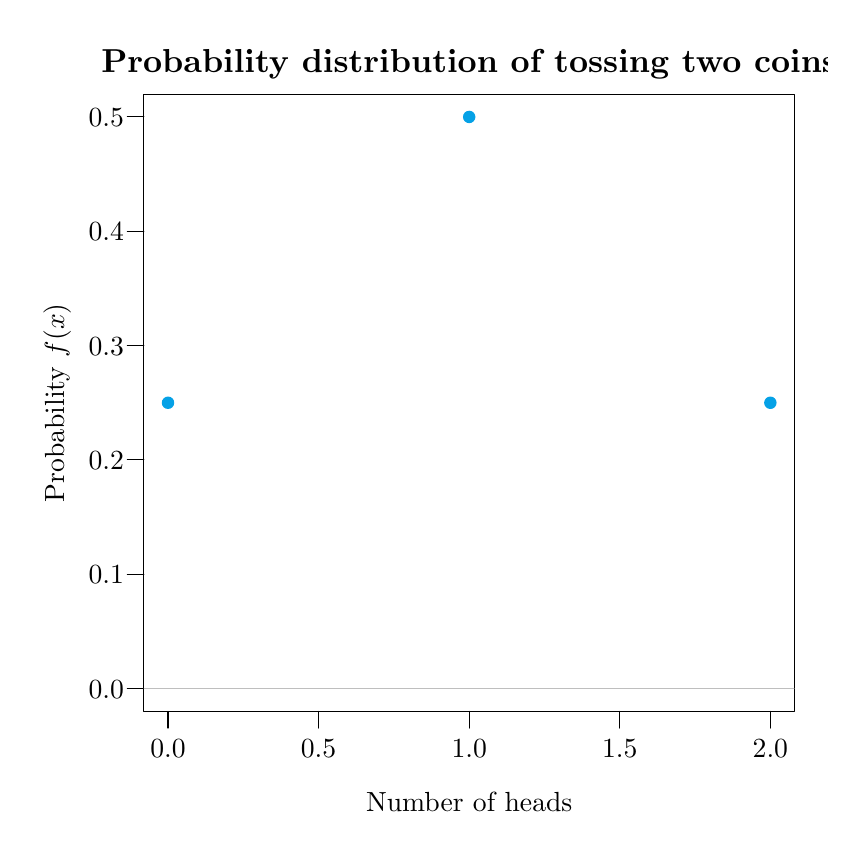
\begin{tikzpicture}[x=1pt,y=1pt]
\definecolor{fillColor}{RGB}{255,255,255}
\path[use as bounding box,fill=fillColor,fill opacity=0.00] (0,0) rectangle (289.08,289.08);
\begin{scope}
\path[clip] ( 42.00, 42.00) rectangle (277.08,265.08);
\definecolor{fillColor}{RGB}{5,161,230}

\path[fill=fillColor] ( 50.71,153.54) circle (  2.25);

\path[fill=fillColor] (159.54,256.82) circle (  2.25);

\path[fill=fillColor] (268.37,153.54) circle (  2.25);
\end{scope}
\begin{scope}
\path[clip] (  0.00,  0.00) rectangle (289.08,289.08);
\definecolor{drawColor}{RGB}{0,0,0}

\path[draw=drawColor,line width= 0.4pt,line join=round,line cap=round] ( 50.71, 42.00) -- (268.37, 42.00);

\path[draw=drawColor,line width= 0.4pt,line join=round,line cap=round] ( 50.71, 42.00) -- ( 50.71, 36.00);

\path[draw=drawColor,line width= 0.4pt,line join=round,line cap=round] (105.12, 42.00) -- (105.12, 36.00);

\path[draw=drawColor,line width= 0.4pt,line join=round,line cap=round] (159.54, 42.00) -- (159.54, 36.00);

\path[draw=drawColor,line width= 0.4pt,line join=round,line cap=round] (213.96, 42.00) -- (213.96, 36.00);

\path[draw=drawColor,line width= 0.4pt,line join=round,line cap=round] (268.37, 42.00) -- (268.37, 36.00);

\node[text=drawColor,anchor=base,inner sep=0pt, outer sep=0pt, scale=  1.00] at ( 50.71, 25.20) {0.0};

\node[text=drawColor,anchor=base,inner sep=0pt, outer sep=0pt, scale=  1.00] at (105.12, 25.20) {0.5};

\node[text=drawColor,anchor=base,inner sep=0pt, outer sep=0pt, scale=  1.00] at (159.54, 25.20) {1.0};

\node[text=drawColor,anchor=base,inner sep=0pt, outer sep=0pt, scale=  1.00] at (213.96, 25.20) {1.5};

\node[text=drawColor,anchor=base,inner sep=0pt, outer sep=0pt, scale=  1.00] at (268.37, 25.20) {2.0};

\path[draw=drawColor,line width= 0.4pt,line join=round,line cap=round] ( 42.00, 50.26) -- ( 42.00,256.82);

\path[draw=drawColor,line width= 0.4pt,line join=round,line cap=round] ( 42.00, 50.26) -- ( 36.00, 50.26);

\path[draw=drawColor,line width= 0.4pt,line join=round,line cap=round] ( 42.00, 91.57) -- ( 36.00, 91.57);

\path[draw=drawColor,line width= 0.4pt,line join=round,line cap=round] ( 42.00,132.88) -- ( 36.00,132.88);

\path[draw=drawColor,line width= 0.4pt,line join=round,line cap=round] ( 42.00,174.20) -- ( 36.00,174.20);

\path[draw=drawColor,line width= 0.4pt,line join=round,line cap=round] ( 42.00,215.51) -- ( 36.00,215.51);

\path[draw=drawColor,line width= 0.4pt,line join=round,line cap=round] ( 42.00,256.82) -- ( 36.00,256.82);

\node[text=drawColor,anchor=base east,inner sep=0pt, outer sep=0pt, scale=  1.00] at ( 34.80, 46.82) {0.0};

\node[text=drawColor,anchor=base east,inner sep=0pt, outer sep=0pt, scale=  1.00] at ( 34.80, 88.13) {0.1};

\node[text=drawColor,anchor=base east,inner sep=0pt, outer sep=0pt, scale=  1.00] at ( 34.80,129.44) {0.2};

\node[text=drawColor,anchor=base east,inner sep=0pt, outer sep=0pt, scale=  1.00] at ( 34.80,170.75) {0.3};

\node[text=drawColor,anchor=base east,inner sep=0pt, outer sep=0pt, scale=  1.00] at ( 34.80,212.06) {0.4};

\node[text=drawColor,anchor=base east,inner sep=0pt, outer sep=0pt, scale=  1.00] at ( 34.80,253.37) {0.5};

\path[draw=drawColor,line width= 0.4pt,line join=round,line cap=round] ( 42.00, 42.00) --
	(277.08, 42.00) --
	(277.08,265.08) --
	( 42.00,265.08) --
	( 42.00, 42.00);
\end{scope}
\begin{scope}
\path[clip] (  0.00,  0.00) rectangle (289.08,289.08);
\definecolor{drawColor}{RGB}{0,0,0}

\node[text=drawColor,anchor=base,inner sep=0pt, outer sep=0pt, scale=  1.20] at (159.54,272.89) {\bfseries Probability distribution of tossing two coins};

\node[text=drawColor,anchor=base,inner sep=0pt, outer sep=0pt, scale=  1.00] at (159.54,  6.00) {Number of heads};

\node[text=drawColor,rotate= 90.00,anchor=base,inner sep=0pt, outer sep=0pt, scale=  1.00] at ( 13.20,153.54) {Probability $f(x)$};
\end{scope}
\begin{scope}
\path[clip] ( 42.00, 42.00) rectangle (277.08,265.08);
\definecolor{drawColor}{RGB}{190,190,190}

\path[draw=drawColor,line width= 0.4pt,line join=round,line cap=round] ( 42.00, 50.26) -- (277.08, 50.26);
\end{scope}
\end{tikzpicture}
}}
\mode<presentation>{\resizebox{0.45\textwidth}{!}{% Created by tikzDevice version 0.10.1 on 2016-04-19 18:05:32
% !TEX encoding = UTF-8 Unicode
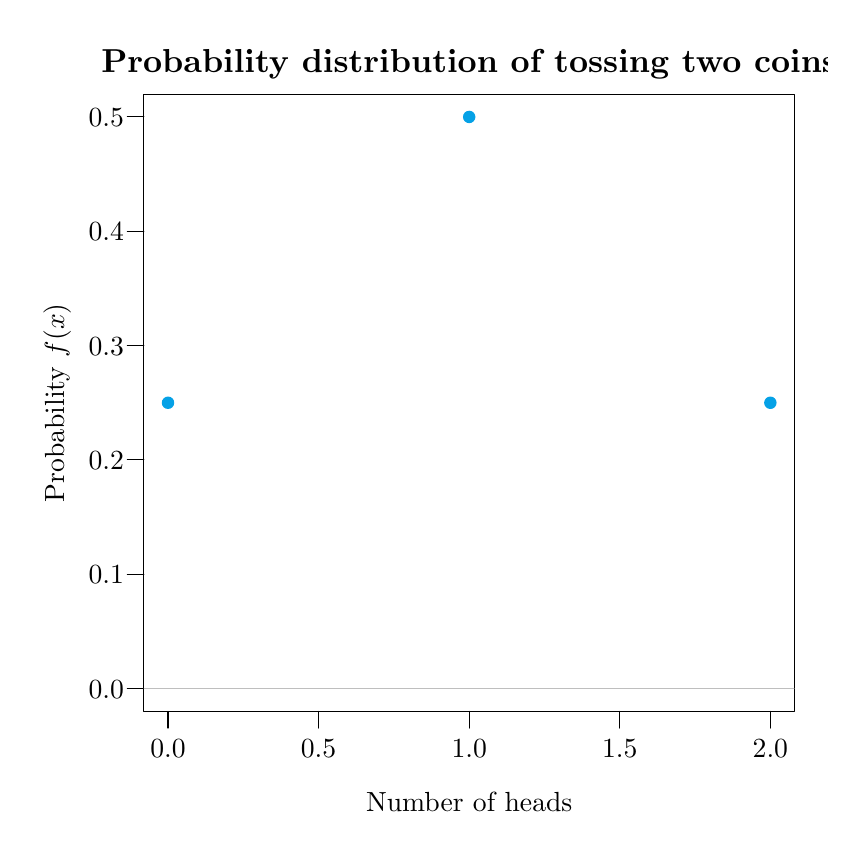
\begin{tikzpicture}[x=1pt,y=1pt]
\definecolor{fillColor}{RGB}{255,255,255}
\path[use as bounding box,fill=fillColor,fill opacity=0.00] (0,0) rectangle (289.08,289.08);
\begin{scope}
\path[clip] ( 42.00, 42.00) rectangle (277.08,265.08);
\definecolor{fillColor}{RGB}{5,161,230}

\path[fill=fillColor] ( 50.71,153.54) circle (  2.25);

\path[fill=fillColor] (159.54,256.82) circle (  2.25);

\path[fill=fillColor] (268.37,153.54) circle (  2.25);
\end{scope}
\begin{scope}
\path[clip] (  0.00,  0.00) rectangle (289.08,289.08);
\definecolor{drawColor}{RGB}{0,0,0}

\path[draw=drawColor,line width= 0.4pt,line join=round,line cap=round] ( 50.71, 42.00) -- (268.37, 42.00);

\path[draw=drawColor,line width= 0.4pt,line join=round,line cap=round] ( 50.71, 42.00) -- ( 50.71, 36.00);

\path[draw=drawColor,line width= 0.4pt,line join=round,line cap=round] (105.12, 42.00) -- (105.12, 36.00);

\path[draw=drawColor,line width= 0.4pt,line join=round,line cap=round] (159.54, 42.00) -- (159.54, 36.00);

\path[draw=drawColor,line width= 0.4pt,line join=round,line cap=round] (213.96, 42.00) -- (213.96, 36.00);

\path[draw=drawColor,line width= 0.4pt,line join=round,line cap=round] (268.37, 42.00) -- (268.37, 36.00);

\node[text=drawColor,anchor=base,inner sep=0pt, outer sep=0pt, scale=  1.00] at ( 50.71, 25.20) {0.0};

\node[text=drawColor,anchor=base,inner sep=0pt, outer sep=0pt, scale=  1.00] at (105.12, 25.20) {0.5};

\node[text=drawColor,anchor=base,inner sep=0pt, outer sep=0pt, scale=  1.00] at (159.54, 25.20) {1.0};

\node[text=drawColor,anchor=base,inner sep=0pt, outer sep=0pt, scale=  1.00] at (213.96, 25.20) {1.5};

\node[text=drawColor,anchor=base,inner sep=0pt, outer sep=0pt, scale=  1.00] at (268.37, 25.20) {2.0};

\path[draw=drawColor,line width= 0.4pt,line join=round,line cap=round] ( 42.00, 50.26) -- ( 42.00,256.82);

\path[draw=drawColor,line width= 0.4pt,line join=round,line cap=round] ( 42.00, 50.26) -- ( 36.00, 50.26);

\path[draw=drawColor,line width= 0.4pt,line join=round,line cap=round] ( 42.00, 91.57) -- ( 36.00, 91.57);

\path[draw=drawColor,line width= 0.4pt,line join=round,line cap=round] ( 42.00,132.88) -- ( 36.00,132.88);

\path[draw=drawColor,line width= 0.4pt,line join=round,line cap=round] ( 42.00,174.20) -- ( 36.00,174.20);

\path[draw=drawColor,line width= 0.4pt,line join=round,line cap=round] ( 42.00,215.51) -- ( 36.00,215.51);

\path[draw=drawColor,line width= 0.4pt,line join=round,line cap=round] ( 42.00,256.82) -- ( 36.00,256.82);

\node[text=drawColor,anchor=base east,inner sep=0pt, outer sep=0pt, scale=  1.00] at ( 34.80, 46.82) {0.0};

\node[text=drawColor,anchor=base east,inner sep=0pt, outer sep=0pt, scale=  1.00] at ( 34.80, 88.13) {0.1};

\node[text=drawColor,anchor=base east,inner sep=0pt, outer sep=0pt, scale=  1.00] at ( 34.80,129.44) {0.2};

\node[text=drawColor,anchor=base east,inner sep=0pt, outer sep=0pt, scale=  1.00] at ( 34.80,170.75) {0.3};

\node[text=drawColor,anchor=base east,inner sep=0pt, outer sep=0pt, scale=  1.00] at ( 34.80,212.06) {0.4};

\node[text=drawColor,anchor=base east,inner sep=0pt, outer sep=0pt, scale=  1.00] at ( 34.80,253.37) {0.5};

\path[draw=drawColor,line width= 0.4pt,line join=round,line cap=round] ( 42.00, 42.00) --
	(277.08, 42.00) --
	(277.08,265.08) --
	( 42.00,265.08) --
	( 42.00, 42.00);
\end{scope}
\begin{scope}
\path[clip] (  0.00,  0.00) rectangle (289.08,289.08);
\definecolor{drawColor}{RGB}{0,0,0}

\node[text=drawColor,anchor=base,inner sep=0pt, outer sep=0pt, scale=  1.20] at (159.54,272.89) {\bfseries Probability distribution of tossing two coins};

\node[text=drawColor,anchor=base,inner sep=0pt, outer sep=0pt, scale=  1.00] at (159.54,  6.00) {Number of heads};

\node[text=drawColor,rotate= 90.00,anchor=base,inner sep=0pt, outer sep=0pt, scale=  1.00] at ( 13.20,153.54) {Probability $f(x)$};
\end{scope}
\begin{scope}
\path[clip] ( 42.00, 42.00) rectangle (277.08,265.08);
\definecolor{drawColor}{RGB}{190,190,190}

\path[draw=drawColor,line width= 0.4pt,line join=round,line cap=round] ( 42.00, 50.26) -- (277.08, 50.26);
\end{scope}
\end{tikzpicture}
}}
&
\tikzsetnextfilename{discrete_random_variables/two_coins_distribution_function}
\mode<article>{\resizebox{0.5\textwidth}{!}{% Created by tikzDevice version 0.10.1 on 2016-04-19 09:52:57
% !TEX encoding = UTF-8 Unicode
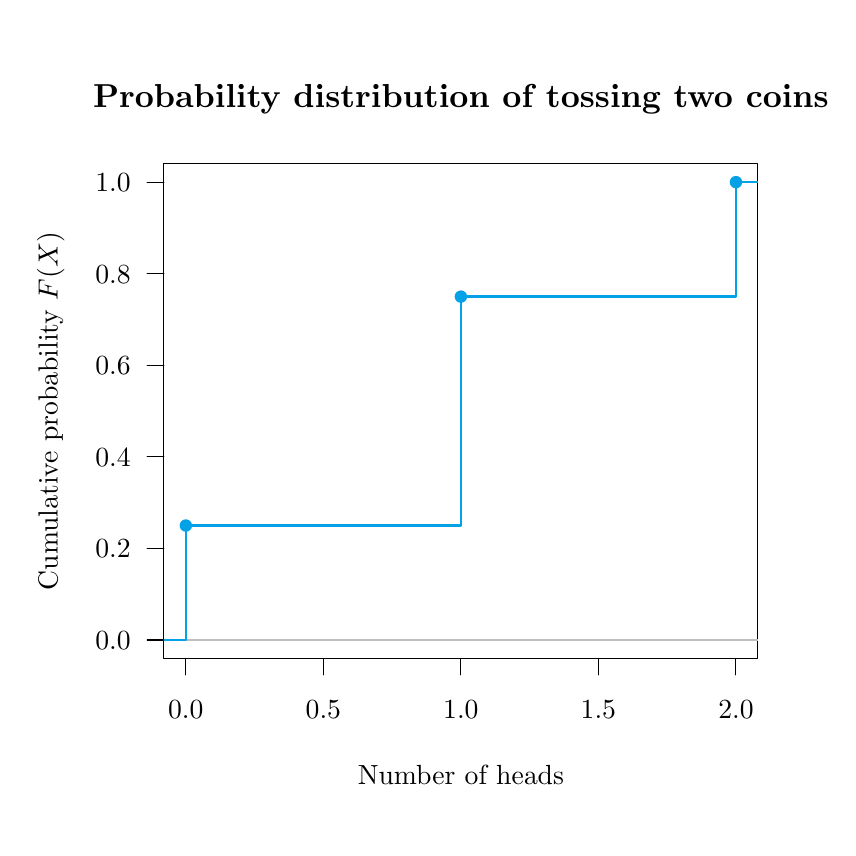
\begin{tikzpicture}[x=1pt,y=1pt]
\definecolor{fillColor}{RGB}{255,255,255}
\path[use as bounding box,fill=fillColor,fill opacity=0.00] (0,0) rectangle (289.08,289.08);
\begin{scope}
\path[clip] ( 49.20, 61.20) rectangle (263.88,239.88);
\definecolor{fillColor}{RGB}{5,161,230}

\path[fill=fillColor] ( 57.15,109.18) circle (  2.25);

\path[fill=fillColor] (156.54,191.90) circle (  2.25);

\path[fill=fillColor] (255.93,233.26) circle (  2.25);
\end{scope}
\begin{scope}
\path[clip] (  0.00,  0.00) rectangle (289.08,289.08);
\definecolor{drawColor}{RGB}{0,0,0}

\path[draw=drawColor,line width= 0.4pt,line join=round,line cap=round] ( 57.15, 61.20) -- (255.93, 61.20);

\path[draw=drawColor,line width= 0.4pt,line join=round,line cap=round] ( 57.15, 61.20) -- ( 57.15, 55.20);

\path[draw=drawColor,line width= 0.4pt,line join=round,line cap=round] (106.85, 61.20) -- (106.85, 55.20);

\path[draw=drawColor,line width= 0.4pt,line join=round,line cap=round] (156.54, 61.20) -- (156.54, 55.20);

\path[draw=drawColor,line width= 0.4pt,line join=round,line cap=round] (206.23, 61.20) -- (206.23, 55.20);

\path[draw=drawColor,line width= 0.4pt,line join=round,line cap=round] (255.93, 61.20) -- (255.93, 55.20);

\node[text=drawColor,anchor=base,inner sep=0pt, outer sep=0pt, scale=  1.00] at ( 57.15, 39.60) {0.0};

\node[text=drawColor,anchor=base,inner sep=0pt, outer sep=0pt, scale=  1.00] at (106.85, 39.60) {0.5};

\node[text=drawColor,anchor=base,inner sep=0pt, outer sep=0pt, scale=  1.00] at (156.54, 39.60) {1.0};

\node[text=drawColor,anchor=base,inner sep=0pt, outer sep=0pt, scale=  1.00] at (206.23, 39.60) {1.5};

\node[text=drawColor,anchor=base,inner sep=0pt, outer sep=0pt, scale=  1.00] at (255.93, 39.60) {2.0};

\path[draw=drawColor,line width= 0.4pt,line join=round,line cap=round] ( 49.20, 67.82) -- ( 49.20,233.26);

\path[draw=drawColor,line width= 0.4pt,line join=round,line cap=round] ( 49.20, 67.82) -- ( 43.20, 67.82);

\path[draw=drawColor,line width= 0.4pt,line join=round,line cap=round] ( 49.20,100.91) -- ( 43.20,100.91);

\path[draw=drawColor,line width= 0.4pt,line join=round,line cap=round] ( 49.20,134.00) -- ( 43.20,134.00);

\path[draw=drawColor,line width= 0.4pt,line join=round,line cap=round] ( 49.20,167.08) -- ( 43.20,167.08);

\path[draw=drawColor,line width= 0.4pt,line join=round,line cap=round] ( 49.20,200.17) -- ( 43.20,200.17);

\path[draw=drawColor,line width= 0.4pt,line join=round,line cap=round] ( 49.20,233.26) -- ( 43.20,233.26);

\node[text=drawColor,anchor=base east,inner sep=0pt, outer sep=0pt, scale=  1.00] at ( 37.20, 64.37) {0.0};

\node[text=drawColor,anchor=base east,inner sep=0pt, outer sep=0pt, scale=  1.00] at ( 37.20, 97.46) {0.2};

\node[text=drawColor,anchor=base east,inner sep=0pt, outer sep=0pt, scale=  1.00] at ( 37.20,130.55) {0.4};

\node[text=drawColor,anchor=base east,inner sep=0pt, outer sep=0pt, scale=  1.00] at ( 37.20,163.64) {0.6};

\node[text=drawColor,anchor=base east,inner sep=0pt, outer sep=0pt, scale=  1.00] at ( 37.20,196.73) {0.8};

\node[text=drawColor,anchor=base east,inner sep=0pt, outer sep=0pt, scale=  1.00] at ( 37.20,229.82) {1.0};

\path[draw=drawColor,line width= 0.4pt,line join=round,line cap=round] ( 49.20, 61.20) --
	(263.88, 61.20) --
	(263.88,239.88) --
	( 49.20,239.88) --
	( 49.20, 61.20);
\end{scope}
\begin{scope}
\path[clip] (  0.00,  0.00) rectangle (289.08,289.08);
\definecolor{drawColor}{RGB}{0,0,0}

\node[text=drawColor,anchor=base,inner sep=0pt, outer sep=0pt, scale=  1.20] at (156.54,260.29) {\bfseries Probability distribution of tossing two coins};

\node[text=drawColor,anchor=base,inner sep=0pt, outer sep=0pt, scale=  1.00] at (156.54, 15.60) {Number of heads};

\node[text=drawColor,rotate= 90.00,anchor=base,inner sep=0pt, outer sep=0pt, scale=  1.00] at ( 10.80,150.54) {Cumulative probability $F(X)$};
\end{scope}
\begin{scope}
\path[clip] ( 49.20, 61.20) rectangle (263.88,239.88);
\definecolor{drawColor}{RGB}{190,190,190}

\path[draw=drawColor,line width= 0.4pt,line join=round,line cap=round] ( 49.20, 67.82) -- (263.88, 67.82);
\definecolor{drawColor}{RGB}{5,161,230}

\path[draw=drawColor,line width= 0.8pt,line join=round,line cap=round] (  0.00, 67.82) --
	( 57.15, 67.82) --
	( 57.15,109.18) --
	(156.54,109.18) --
	(156.54,191.90) --
	(255.93,191.90) --
	(255.93,233.26) --
	(289.08,233.26);
\end{scope}
\end{tikzpicture}
}}
\mode<presentation>{\resizebox{0.45\textwidth}{!}{% Created by tikzDevice version 0.10.1 on 2016-04-19 09:52:57
% !TEX encoding = UTF-8 Unicode
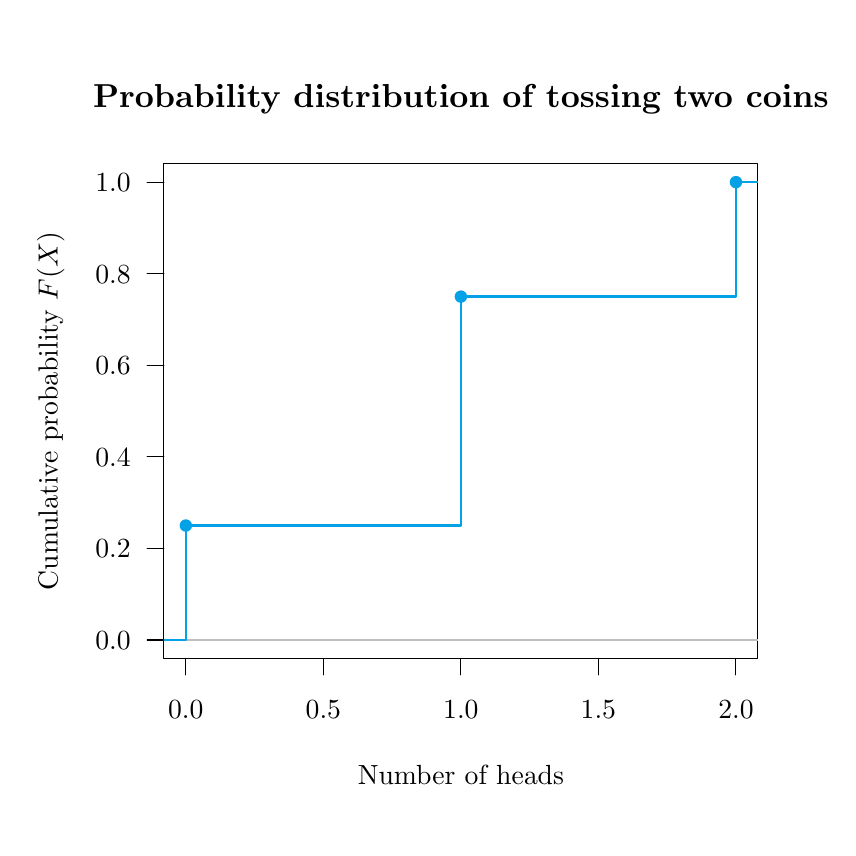
\begin{tikzpicture}[x=1pt,y=1pt]
\definecolor{fillColor}{RGB}{255,255,255}
\path[use as bounding box,fill=fillColor,fill opacity=0.00] (0,0) rectangle (289.08,289.08);
\begin{scope}
\path[clip] ( 49.20, 61.20) rectangle (263.88,239.88);
\definecolor{fillColor}{RGB}{5,161,230}

\path[fill=fillColor] ( 57.15,109.18) circle (  2.25);

\path[fill=fillColor] (156.54,191.90) circle (  2.25);

\path[fill=fillColor] (255.93,233.26) circle (  2.25);
\end{scope}
\begin{scope}
\path[clip] (  0.00,  0.00) rectangle (289.08,289.08);
\definecolor{drawColor}{RGB}{0,0,0}

\path[draw=drawColor,line width= 0.4pt,line join=round,line cap=round] ( 57.15, 61.20) -- (255.93, 61.20);

\path[draw=drawColor,line width= 0.4pt,line join=round,line cap=round] ( 57.15, 61.20) -- ( 57.15, 55.20);

\path[draw=drawColor,line width= 0.4pt,line join=round,line cap=round] (106.85, 61.20) -- (106.85, 55.20);

\path[draw=drawColor,line width= 0.4pt,line join=round,line cap=round] (156.54, 61.20) -- (156.54, 55.20);

\path[draw=drawColor,line width= 0.4pt,line join=round,line cap=round] (206.23, 61.20) -- (206.23, 55.20);

\path[draw=drawColor,line width= 0.4pt,line join=round,line cap=round] (255.93, 61.20) -- (255.93, 55.20);

\node[text=drawColor,anchor=base,inner sep=0pt, outer sep=0pt, scale=  1.00] at ( 57.15, 39.60) {0.0};

\node[text=drawColor,anchor=base,inner sep=0pt, outer sep=0pt, scale=  1.00] at (106.85, 39.60) {0.5};

\node[text=drawColor,anchor=base,inner sep=0pt, outer sep=0pt, scale=  1.00] at (156.54, 39.60) {1.0};

\node[text=drawColor,anchor=base,inner sep=0pt, outer sep=0pt, scale=  1.00] at (206.23, 39.60) {1.5};

\node[text=drawColor,anchor=base,inner sep=0pt, outer sep=0pt, scale=  1.00] at (255.93, 39.60) {2.0};

\path[draw=drawColor,line width= 0.4pt,line join=round,line cap=round] ( 49.20, 67.82) -- ( 49.20,233.26);

\path[draw=drawColor,line width= 0.4pt,line join=round,line cap=round] ( 49.20, 67.82) -- ( 43.20, 67.82);

\path[draw=drawColor,line width= 0.4pt,line join=round,line cap=round] ( 49.20,100.91) -- ( 43.20,100.91);

\path[draw=drawColor,line width= 0.4pt,line join=round,line cap=round] ( 49.20,134.00) -- ( 43.20,134.00);

\path[draw=drawColor,line width= 0.4pt,line join=round,line cap=round] ( 49.20,167.08) -- ( 43.20,167.08);

\path[draw=drawColor,line width= 0.4pt,line join=round,line cap=round] ( 49.20,200.17) -- ( 43.20,200.17);

\path[draw=drawColor,line width= 0.4pt,line join=round,line cap=round] ( 49.20,233.26) -- ( 43.20,233.26);

\node[text=drawColor,anchor=base east,inner sep=0pt, outer sep=0pt, scale=  1.00] at ( 37.20, 64.37) {0.0};

\node[text=drawColor,anchor=base east,inner sep=0pt, outer sep=0pt, scale=  1.00] at ( 37.20, 97.46) {0.2};

\node[text=drawColor,anchor=base east,inner sep=0pt, outer sep=0pt, scale=  1.00] at ( 37.20,130.55) {0.4};

\node[text=drawColor,anchor=base east,inner sep=0pt, outer sep=0pt, scale=  1.00] at ( 37.20,163.64) {0.6};

\node[text=drawColor,anchor=base east,inner sep=0pt, outer sep=0pt, scale=  1.00] at ( 37.20,196.73) {0.8};

\node[text=drawColor,anchor=base east,inner sep=0pt, outer sep=0pt, scale=  1.00] at ( 37.20,229.82) {1.0};

\path[draw=drawColor,line width= 0.4pt,line join=round,line cap=round] ( 49.20, 61.20) --
	(263.88, 61.20) --
	(263.88,239.88) --
	( 49.20,239.88) --
	( 49.20, 61.20);
\end{scope}
\begin{scope}
\path[clip] (  0.00,  0.00) rectangle (289.08,289.08);
\definecolor{drawColor}{RGB}{0,0,0}

\node[text=drawColor,anchor=base,inner sep=0pt, outer sep=0pt, scale=  1.20] at (156.54,260.29) {\bfseries Probability distribution of tossing two coins};

\node[text=drawColor,anchor=base,inner sep=0pt, outer sep=0pt, scale=  1.00] at (156.54, 15.60) {Number of heads};

\node[text=drawColor,rotate= 90.00,anchor=base,inner sep=0pt, outer sep=0pt, scale=  1.00] at ( 10.80,150.54) {Cumulative probability $F(X)$};
\end{scope}
\begin{scope}
\path[clip] ( 49.20, 61.20) rectangle (263.88,239.88);
\definecolor{drawColor}{RGB}{190,190,190}

\path[draw=drawColor,line width= 0.4pt,line join=round,line cap=round] ( 49.20, 67.82) -- (263.88, 67.82);
\definecolor{drawColor}{RGB}{5,161,230}

\path[draw=drawColor,line width= 0.8pt,line join=round,line cap=round] (  0.00, 67.82) --
	( 57.15, 67.82) --
	( 57.15,109.18) --
	(156.54,109.18) --
	(156.54,191.90) --
	(255.93,191.90) --
	(255.93,233.26) --
	(289.08,233.26);
\end{scope}
\end{tikzpicture}
}}
\end{tabular}
\end{center} 
\end{frame}


%---------------------------------------------------------------------slide----
\begin{frame}
\frametitle{Population statistics}
The same way we use sample statistics to describe the sample frequency distribution of a variable, we use
population statistics to describe the probability distribution of a random variable in the whole population.

The population statistics definition is analogous to the to the sample statistics definition, but using probabilities
instead of relative frequencies. 

The most important are \footnote{To distinguish population statistics from sample statistics we use Greek letters}:
\begin{itemize}
\item \structure{Mean}:
\[
\mu = E(X) = \sum_{i=1}^n x_i f(x_i)
\]
\item \structure{Variance}:
\[
\sigma^2 = Var(X) = \sum_{i=1}^n x_i^2 f(x_i) -\mu^2
\]
\item \structure{Standard deviation}:
\[
\sigma = +\sqrt{\sigma^2}
\]
\end{itemize}
\end{frame}


%---------------------------------------------------------------------slide----
\begin{frame}
\frametitle{Population statistics}
\framesubtitle{Example of tossing two coins}
In the random experiment of tossing two coins the probability distribution is  
\[
\begin{array}{|c|ccc|}
\hline
X & 0 & 1 & 2\\ \hline
f(x) & 0.25 & 0.5 & 0.25\\
\hline
F(x) & 0.25 & 0.75 & 1 \\
\hline
\end{array}
\]

The main population statistics are 
\begin{align*}
\mu &= \sum_{i=1}^n x_i f(x_i) = 0\cdot 0.25 + 1\cdot 0.5 + 2\cdot 0.25 = 1 \mbox{ heads},\\
\sigma^2 &= \sum_{i=1}^n x_i^2 f(x_i) -\mu^2 = (0^0\cdot 0.25 + 1^2\cdot 0.5 + 2^2\cdot 0.25) - 1^2 = 0.5 \mbox{
heads}^2,\\
\sigma &= +\sqrt{0.5} = 0.71 \mbox{ heads}.
\end{align*}
\end{frame}


%---------------------------------------------------------------------slide----
\begin{frame}
\frametitle{Discrete probability distribution models}
According to the type of experiment where the random variable is measured, there are different probability distributions
models. 
The most common are

\begin{itemize}
\item Discrete uniform
\item Binomial
\item Poisson 
\end{itemize}
\end{frame}


\subsection{Discrete uniform distribution}

% ---------------------------------------------------------------------slide----
\begin{frame}
\frametitle{Discrete uniform probability distribution model $U(a,b)$}
When all the values of a random variable $X$ have equal probability, the probability distribution of $X$
is uniform.

\begin{definition}[Discrete uniform distribution $U(a,b)$]
A discrete random variable $X$ follows a \emph{discrete uniform distribution model} with parameters $a$ and $b$, noted 
$X\sim U(a,b)$, if its range is $Ran(X) = \{a, a+1, \ldots,b\}$ and its probability function is
\[f(x)=\frac{1}{b-a+1}.\]
\end{definition}

Observe that $a$ and $b$ are the minimum and the maximum of the range respectively. 

The mean and the variance are
\[
\mu = \sum_{i=0}^{b-a}\frac{a+i}{b-a+1}=\frac{a+b}{2} \qquad \sigma^2 =\sum_{i=0}^{b-a}\frac{(a+i-\mu)^2}{b-a+1}=
\frac{(b-a+1)^2-1}{12}
\]
\end{frame}


%---------------------------------------------------------------------slide----
\begin{frame}
\frametitle{Discrete uniform probability distribution model $U(a,b)$}
\framesubtitle{Example of rolling a dice}
The variable that measures the outcome of rolling a dice follows a discrete uniform distribution model $U(1,6)$.
\begin{center}
\scalebox{0.65}{% Created by tikzDevice version 0.10.1 on 2016-04-19 09:52:58
% !TEX encoding = UTF-8 Unicode
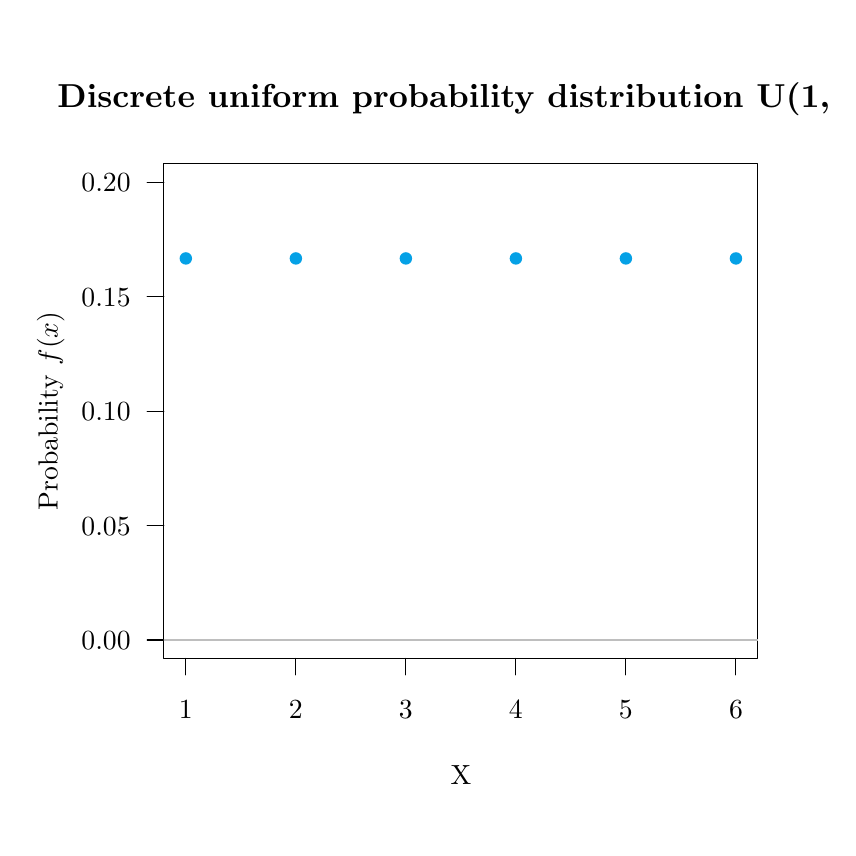
\begin{tikzpicture}[x=1pt,y=1pt]
\definecolor{fillColor}{RGB}{255,255,255}
\path[use as bounding box,fill=fillColor,fill opacity=0.00] (0,0) rectangle (289.08,289.08);
\begin{scope}
\path[clip] ( 49.20, 61.20) rectangle (263.88,239.88);
\definecolor{fillColor}{RGB}{5,161,230}

\path[fill=fillColor] ( 57.15,205.69) circle (  2.25);

\path[fill=fillColor] ( 96.91,205.69) circle (  2.25);

\path[fill=fillColor] (136.66,205.69) circle (  2.25);

\path[fill=fillColor] (176.42,205.69) circle (  2.25);

\path[fill=fillColor] (216.17,205.69) circle (  2.25);

\path[fill=fillColor] (255.93,205.69) circle (  2.25);
\end{scope}
\begin{scope}
\path[clip] (  0.00,  0.00) rectangle (289.08,289.08);
\definecolor{drawColor}{RGB}{0,0,0}

\path[draw=drawColor,line width= 0.4pt,line join=round,line cap=round] ( 57.15, 61.20) -- (255.93, 61.20);

\path[draw=drawColor,line width= 0.4pt,line join=round,line cap=round] ( 57.15, 61.20) -- ( 57.15, 55.20);

\path[draw=drawColor,line width= 0.4pt,line join=round,line cap=round] ( 96.91, 61.20) -- ( 96.91, 55.20);

\path[draw=drawColor,line width= 0.4pt,line join=round,line cap=round] (136.66, 61.20) -- (136.66, 55.20);

\path[draw=drawColor,line width= 0.4pt,line join=round,line cap=round] (176.42, 61.20) -- (176.42, 55.20);

\path[draw=drawColor,line width= 0.4pt,line join=round,line cap=round] (216.17, 61.20) -- (216.17, 55.20);

\path[draw=drawColor,line width= 0.4pt,line join=round,line cap=round] (255.93, 61.20) -- (255.93, 55.20);

\node[text=drawColor,anchor=base,inner sep=0pt, outer sep=0pt, scale=  1.00] at ( 57.15, 39.60) {1};

\node[text=drawColor,anchor=base,inner sep=0pt, outer sep=0pt, scale=  1.00] at ( 96.91, 39.60) {2};

\node[text=drawColor,anchor=base,inner sep=0pt, outer sep=0pt, scale=  1.00] at (136.66, 39.60) {3};

\node[text=drawColor,anchor=base,inner sep=0pt, outer sep=0pt, scale=  1.00] at (176.42, 39.60) {4};

\node[text=drawColor,anchor=base,inner sep=0pt, outer sep=0pt, scale=  1.00] at (216.17, 39.60) {5};

\node[text=drawColor,anchor=base,inner sep=0pt, outer sep=0pt, scale=  1.00] at (255.93, 39.60) {6};

\path[draw=drawColor,line width= 0.4pt,line join=round,line cap=round] ( 49.20, 67.82) -- ( 49.20,233.26);

\path[draw=drawColor,line width= 0.4pt,line join=round,line cap=round] ( 49.20, 67.82) -- ( 43.20, 67.82);

\path[draw=drawColor,line width= 0.4pt,line join=round,line cap=round] ( 49.20,109.18) -- ( 43.20,109.18);

\path[draw=drawColor,line width= 0.4pt,line join=round,line cap=round] ( 49.20,150.54) -- ( 43.20,150.54);

\path[draw=drawColor,line width= 0.4pt,line join=round,line cap=round] ( 49.20,191.90) -- ( 43.20,191.90);

\path[draw=drawColor,line width= 0.4pt,line join=round,line cap=round] ( 49.20,233.26) -- ( 43.20,233.26);

\node[text=drawColor,anchor=base east,inner sep=0pt, outer sep=0pt, scale=  1.00] at ( 37.20, 64.37) {0.00};

\node[text=drawColor,anchor=base east,inner sep=0pt, outer sep=0pt, scale=  1.00] at ( 37.20,105.73) {0.05};

\node[text=drawColor,anchor=base east,inner sep=0pt, outer sep=0pt, scale=  1.00] at ( 37.20,147.10) {0.10};

\node[text=drawColor,anchor=base east,inner sep=0pt, outer sep=0pt, scale=  1.00] at ( 37.20,188.46) {0.15};

\node[text=drawColor,anchor=base east,inner sep=0pt, outer sep=0pt, scale=  1.00] at ( 37.20,229.82) {0.20};

\path[draw=drawColor,line width= 0.4pt,line join=round,line cap=round] ( 49.20, 61.20) --
	(263.88, 61.20) --
	(263.88,239.88) --
	( 49.20,239.88) --
	( 49.20, 61.20);
\end{scope}
\begin{scope}
\path[clip] (  0.00,  0.00) rectangle (289.08,289.08);
\definecolor{drawColor}{RGB}{0,0,0}

\node[text=drawColor,anchor=base,inner sep=0pt, outer sep=0pt, scale=  1.20] at (156.54,260.29) {\bfseries Discrete uniform probability distribution U(1,6)};

\node[text=drawColor,anchor=base,inner sep=0pt, outer sep=0pt, scale=  1.00] at (156.54, 15.60) {X};

\node[text=drawColor,rotate= 90.00,anchor=base,inner sep=0pt, outer sep=0pt, scale=  1.00] at ( 10.80,150.54) {Probability $f(x)$};
\end{scope}
\begin{scope}
\path[clip] ( 49.20, 61.20) rectangle (263.88,239.88);
\definecolor{drawColor}{RGB}{190,190,190}

\path[draw=drawColor,line width= 0.4pt,line join=round,line cap=round] ( 49.20, 67.82) -- (263.88, 67.82);
\end{scope}
\end{tikzpicture}
}
\end{center} 
\end{frame}


\subsection{Binomial distribution}

%---------------------------------------------------------------------slide----
\begin{frame}
\frametitle{Binomial distribution}
Usually the binomial distribution correspond to a variable measured in a random experiment with the following features:
\begin{itemize}
\item The experiment consist in a sequence of $n$ repetitions of the same trial.
\item Each trial is repeated in identical conditions and produces two possible outcomes known as \emph{Success} or
\emph{Failure}.
\item The trials are independent among them.
\item The probability of Success is the same in all the trials and is $P(\mbox{Success})=p$.
\end{itemize}

Under these conditions, the discrete random variable $X$ that measures the number of successes in the $n$ trials follows
a \emph{binomial distribution model} with parameters $n$ and $p$.
\end{frame}


%---------------------------------------------------------------------slide----
\begin{frame}
\frametitle{Binomial distribution model $B(n,p)$}
\begin{definition}[Binomial distribution $(B(n,p)$]
A discrete random variable $X$ follows a \emph{binomial distribution model} with parameters $n$ and $p$, noted 
$X\sim B(n,p)$, if its range is $Ran(X) = \{0,1,\ldots,n\}$ and its probability function is
\[
f(x) = \binom{n}{x}p^x(1-p)^{n-x} = \frac{n!}{x!(n-x)!}p^x(1-p)^{n-x}.
\]
\end{definition}

Observe that $n$ is known as the number of repetitions of a trial and $p$ is known as the probability of Success in
every repetition. 

The mean and the variance are
\[
\mu = n\cdot p \qquad \sigma^2 = n\cdot p\cdot (1-p).
\]
\end{frame}


%---------------------------------------------------------------------slide----
\begin{frame}
\frametitle{Binomial distribution model $B(n,p)$}
\framesubtitle{Example of tossing 10 coins}
The variable that measures the number of heads after tossing 10 coins follows a binomial distribution model $B(10,0.5)$.
\begin{center}
\scalebox{0.65}{% Created by tikzDevice version 0.10.1 on 2016-04-19 09:54:30
% !TEX encoding = UTF-8 Unicode
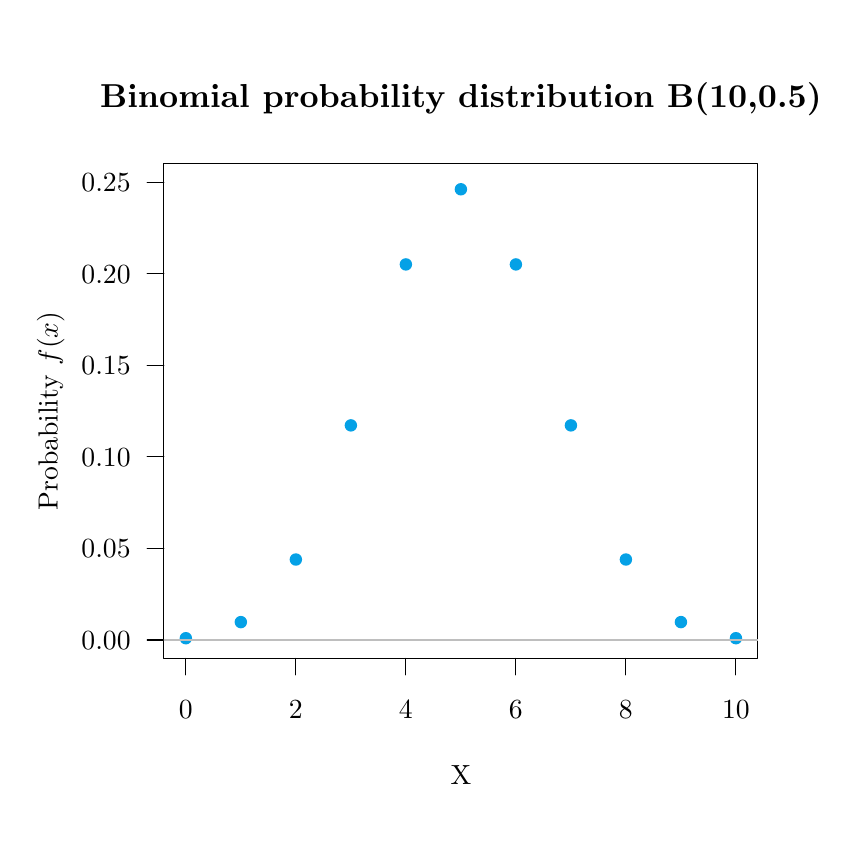
\begin{tikzpicture}[x=1pt,y=1pt]
\definecolor{fillColor}{RGB}{255,255,255}
\path[use as bounding box,fill=fillColor,fill opacity=0.00] (0,0) rectangle (289.08,289.08);
\begin{scope}
\path[clip] ( 49.20, 61.20) rectangle (263.88,239.88);
\definecolor{fillColor}{RGB}{5,161,230}

\path[fill=fillColor] ( 57.15, 68.46) circle (  2.25);

\path[fill=fillColor] ( 77.03, 74.28) circle (  2.25);

\path[fill=fillColor] ( 96.91, 96.90) circle (  2.25);

\path[fill=fillColor] (116.78,145.37) circle (  2.25);

\path[fill=fillColor] (136.66,203.53) circle (  2.25);

\path[fill=fillColor] (156.54,230.68) circle (  2.25);

\path[fill=fillColor] (176.42,203.53) circle (  2.25);

\path[fill=fillColor] (196.30,145.37) circle (  2.25);

\path[fill=fillColor] (216.17, 96.90) circle (  2.25);

\path[fill=fillColor] (236.05, 74.28) circle (  2.25);

\path[fill=fillColor] (255.93, 68.46) circle (  2.25);
\end{scope}
\begin{scope}
\path[clip] (  0.00,  0.00) rectangle (289.08,289.08);
\definecolor{drawColor}{RGB}{0,0,0}

\path[draw=drawColor,line width= 0.4pt,line join=round,line cap=round] ( 57.15, 61.20) -- (255.93, 61.20);

\path[draw=drawColor,line width= 0.4pt,line join=round,line cap=round] ( 57.15, 61.20) -- ( 57.15, 55.20);

\path[draw=drawColor,line width= 0.4pt,line join=round,line cap=round] ( 96.91, 61.20) -- ( 96.91, 55.20);

\path[draw=drawColor,line width= 0.4pt,line join=round,line cap=round] (136.66, 61.20) -- (136.66, 55.20);

\path[draw=drawColor,line width= 0.4pt,line join=round,line cap=round] (176.42, 61.20) -- (176.42, 55.20);

\path[draw=drawColor,line width= 0.4pt,line join=round,line cap=round] (216.17, 61.20) -- (216.17, 55.20);

\path[draw=drawColor,line width= 0.4pt,line join=round,line cap=round] (255.93, 61.20) -- (255.93, 55.20);

\node[text=drawColor,anchor=base,inner sep=0pt, outer sep=0pt, scale=  1.00] at ( 57.15, 39.60) {0};

\node[text=drawColor,anchor=base,inner sep=0pt, outer sep=0pt, scale=  1.00] at ( 96.91, 39.60) {2};

\node[text=drawColor,anchor=base,inner sep=0pt, outer sep=0pt, scale=  1.00] at (136.66, 39.60) {4};

\node[text=drawColor,anchor=base,inner sep=0pt, outer sep=0pt, scale=  1.00] at (176.42, 39.60) {6};

\node[text=drawColor,anchor=base,inner sep=0pt, outer sep=0pt, scale=  1.00] at (216.17, 39.60) {8};

\node[text=drawColor,anchor=base,inner sep=0pt, outer sep=0pt, scale=  1.00] at (255.93, 39.60) {10};

\path[draw=drawColor,line width= 0.4pt,line join=round,line cap=round] ( 49.20, 67.82) -- ( 49.20,233.26);

\path[draw=drawColor,line width= 0.4pt,line join=round,line cap=round] ( 49.20, 67.82) -- ( 43.20, 67.82);

\path[draw=drawColor,line width= 0.4pt,line join=round,line cap=round] ( 49.20,100.91) -- ( 43.20,100.91);

\path[draw=drawColor,line width= 0.4pt,line join=round,line cap=round] ( 49.20,134.00) -- ( 43.20,134.00);

\path[draw=drawColor,line width= 0.4pt,line join=round,line cap=round] ( 49.20,167.08) -- ( 43.20,167.08);

\path[draw=drawColor,line width= 0.4pt,line join=round,line cap=round] ( 49.20,200.17) -- ( 43.20,200.17);

\path[draw=drawColor,line width= 0.4pt,line join=round,line cap=round] ( 49.20,233.26) -- ( 43.20,233.26);

\node[text=drawColor,anchor=base east,inner sep=0pt, outer sep=0pt, scale=  1.00] at ( 37.20, 64.37) {0.00};

\node[text=drawColor,anchor=base east,inner sep=0pt, outer sep=0pt, scale=  1.00] at ( 37.20, 97.46) {0.05};

\node[text=drawColor,anchor=base east,inner sep=0pt, outer sep=0pt, scale=  1.00] at ( 37.20,130.55) {0.10};

\node[text=drawColor,anchor=base east,inner sep=0pt, outer sep=0pt, scale=  1.00] at ( 37.20,163.64) {0.15};

\node[text=drawColor,anchor=base east,inner sep=0pt, outer sep=0pt, scale=  1.00] at ( 37.20,196.73) {0.20};

\node[text=drawColor,anchor=base east,inner sep=0pt, outer sep=0pt, scale=  1.00] at ( 37.20,229.82) {0.25};

\path[draw=drawColor,line width= 0.4pt,line join=round,line cap=round] ( 49.20, 61.20) --
	(263.88, 61.20) --
	(263.88,239.88) --
	( 49.20,239.88) --
	( 49.20, 61.20);
\end{scope}
\begin{scope}
\path[clip] (  0.00,  0.00) rectangle (289.08,289.08);
\definecolor{drawColor}{RGB}{0,0,0}

\node[text=drawColor,anchor=base,inner sep=0pt, outer sep=0pt, scale=  1.20] at (156.54,260.29) {\bfseries Binomial probability distribution B(10,0.5)};

\node[text=drawColor,anchor=base,inner sep=0pt, outer sep=0pt, scale=  1.00] at (156.54, 15.60) {X};

\node[text=drawColor,rotate= 90.00,anchor=base,inner sep=0pt, outer sep=0pt, scale=  1.00] at ( 10.80,150.54) {Probability $f(x)$};
\end{scope}
\begin{scope}
\path[clip] ( 49.20, 61.20) rectangle (263.88,239.88);
\definecolor{drawColor}{RGB}{190,190,190}

\path[draw=drawColor,line width= 0.4pt,line join=round,line cap=round] ( 49.20, 67.82) -- (263.88, 67.82);
\end{scope}
\end{tikzpicture}
}
\end{center}
\end{frame}


%---------------------------------------------------------------------slide----
\begin{frame}
\frametitle{Binomial distribution model $B(n,p)$}
\framesubtitle{Example of tossing 10 coins}
If $X\sim B(10,\,0.5)$ is the random variable that measures the number of heads after tossing 10 coins, then
\begin{itemize}
\item The probability of getting 4 heads is 
\[
f(4) = \binom{10}{4}0.5^4 (1-0.5)^{10-4} = \frac{10!}{4!6!}0.5^40.5^6 = 210\cdot 0.5^{10} = 0.2051.
\]
\item The probability of getting 2 or less heads is
\begin{align*}
F(2) &= f(0) +f(1) + f(2) =\\
&= \binom{10}{0}0.5^0 (1-0.5)^{10-0} + \binom{10}{1}0.5^1 (1-0.5)^{10-1} + \binom{10}{2}0.5^2 (1-0.5)^{10-2} =\\
&= 0.0547.
\end{align*}
\item And the expected number of heads is
\[ \mu = 10\cdot 0.5 = 5 \mbox{ heads}.\]
\end{itemize}
\end{frame}


%---------------------------------------------------------------------slide----
\begin{frame}
\frametitle{Binomial distribution function $B(n,p)$}
\framesubtitle{Example of random sampling with replacement}
In a population there are a 40\% of smokers. 
The variable $X$ that measures the number of smokers in a random sample with replacement of 3 persons follows a
binomial distribution model $X\sim B(3,\,0.4)$.

\begin{center}
\tikzsetnextfilename{discrete_random_variables/binomial_probability_space}
\mode<article>{\resizebox{0.7\textwidth}{!}{% Author: Alfredo Sánchez Alberca (asalber@ceu.es)

\begin{tikzpicture}[
grow'=right,
% sloped,
level 1/.style ={level distance=2cm, sibling distance=3.2cm, parent anchor=east, child anchor=west},
level 2/.style ={level distance=2cm, sibling distance=1.6cm},
level 3/.style ={level distance=2cm, sibling distance=0.8cm},
level 4/.style ={level distance=1.5cm, sibling distance=0.8cm, dashed},
level 5/.style ={level distance=3cm, sibling distance=0.8cm, dashed},
prob/.style={font=\footnotesize,above}
]

\node (root) {}
	child {node {$S$}
		child {node {$S$}
	   		child {node {$S$}
				child {node{\only<2>{\color{color2}}$(S,S,S)$}
					child {node {$0.064$} edge from parent node[prob] {$0.4\cdot 0.4\cdot 0.4$}} 
				}
				edge from parent node[prob] {$0.4$}
			}
			child {node {$\bar S$}
				child {node{\only<3>{\color{color2}}$(S,S,\bar S)$}
					child {node {$0.096$} edge from parent node[prob] {$0.4\cdot 0.4\cdot 0.6$}}
				}
				edge from parent node[prob,below] {$0.6$}
			}
			edge from parent node[prob] {$0.4$}
		}
		child {node {M}
	   		child {node {$S$}
				child {node{\only<3>{\color{color2}}$(S,\bar S,S)$}
					child {node{$0.096$} edge from parent node[prob] {$0.4\cdot 0.6\cdot 0.4$}}
				}
				edge from parent node[prob] {$0.4$}
			}
			child {node {$\bar S$}
				child {node{\only<4>{\color{color2}}$(S,\bar S,\bar S)$}
					child {node{$0.144$} edge from parent node[prob] {$0.4\cdot 0.6\cdot 0.6$}}
				}
				edge from parent node[prob,below] {$0.6$}
			}
			edge from parent node[prob,below] {$0.6$}
		}
		edge from parent node[prob,left] {$0.6$}
	}
	child {node {$\bar S$}
		child {node {S}
	   		child {node {S}
				child {node{\only<3>{\color{color2}}$(\bar S,S,S)$}
					child {node {$0.096$} edge from parent node[prob] {$0.6\cdot 0.4\cdot 0.4$}} 
				}
				edge from parent node[prob] {$0.4$}
			}
			child {node {$\bar S$}
				child {node{\only<4>{\color{color2}}$(\bar S,S,\bar S)$}
					child {node {$0.144$} edge from parent node[prob] {$0.6\cdot 0.4\cdot 0.6$}}
				}
				edge from parent node[prob,below] {$0.6$}
			}
			edge from parent node[prob] {$0.4$}
		}
		child {node {$\bar X$}
	   		child {node {S}
				child {node{\only<4>{\color{color2}}$(\bar S,\bar S,S)$}
					child {node{$0.144$} edge from parent node[prob] {$0.6\cdot 0.6\cdot 0.4$}}
				}
				edge from parent node[prob] {$0.4$}
			}
			child {node {$\bar S$}
				child {node{\only<5>{\color{color2}}$(\bar S,\bar S,\bar S)$}
					child {node{$0.216$} edge from parent node[prob] {$0.6\cdot 0.6\cdot 0.6$}}
				}
				edge from parent node[prob,below] {$0.6$}
			}
			edge from parent node[prob,below] {$0.6$}
		}
		edge from parent node[prob,left] {$0.6$}
	};

\begin{scope}[every node/.style={text width=2cm, align=center, anchor=center, font=\bfseries,}]
\node[above= 0.5cm of root-1-1-1-1-1] (labels-level) {Probability};
\node[at =(labels-level-|root-1)] {Person 1};
\node[at =(labels-level-|root-1-1)] {Person 2};
\node[at =(labels-level-|root-1-1-1)] {Person 3};
\node[at =(labels-level-|root-1-1-1-1)]{$\Omega$};
\end{scope}
\end{tikzpicture}
}}
\mode<presentation>{\resizebox{0.65\textwidth}{!}{% Author: Alfredo Sánchez Alberca (asalber@ceu.es)

\begin{tikzpicture}[
grow'=right,
% sloped,
level 1/.style ={level distance=2cm, sibling distance=3.2cm, parent anchor=east, child anchor=west},
level 2/.style ={level distance=2cm, sibling distance=1.6cm},
level 3/.style ={level distance=2cm, sibling distance=0.8cm},
level 4/.style ={level distance=1.5cm, sibling distance=0.8cm, dashed},
level 5/.style ={level distance=3cm, sibling distance=0.8cm, dashed},
prob/.style={font=\footnotesize,above}
]

\node (root) {}
	child {node {$S$}
		child {node {$S$}
	   		child {node {$S$}
				child {node{\only<2>{\color{color2}}$(S,S,S)$}
					child {node {$0.064$} edge from parent node[prob] {$0.4\cdot 0.4\cdot 0.4$}} 
				}
				edge from parent node[prob] {$0.4$}
			}
			child {node {$\bar S$}
				child {node{\only<3>{\color{color2}}$(S,S,\bar S)$}
					child {node {$0.096$} edge from parent node[prob] {$0.4\cdot 0.4\cdot 0.6$}}
				}
				edge from parent node[prob,below] {$0.6$}
			}
			edge from parent node[prob] {$0.4$}
		}
		child {node {M}
	   		child {node {$S$}
				child {node{\only<3>{\color{color2}}$(S,\bar S,S)$}
					child {node{$0.096$} edge from parent node[prob] {$0.4\cdot 0.6\cdot 0.4$}}
				}
				edge from parent node[prob] {$0.4$}
			}
			child {node {$\bar S$}
				child {node{\only<4>{\color{color2}}$(S,\bar S,\bar S)$}
					child {node{$0.144$} edge from parent node[prob] {$0.4\cdot 0.6\cdot 0.6$}}
				}
				edge from parent node[prob,below] {$0.6$}
			}
			edge from parent node[prob,below] {$0.6$}
		}
		edge from parent node[prob,left] {$0.6$}
	}
	child {node {$\bar S$}
		child {node {S}
	   		child {node {S}
				child {node{\only<3>{\color{color2}}$(\bar S,S,S)$}
					child {node {$0.096$} edge from parent node[prob] {$0.6\cdot 0.4\cdot 0.4$}} 
				}
				edge from parent node[prob] {$0.4$}
			}
			child {node {$\bar S$}
				child {node{\only<4>{\color{color2}}$(\bar S,S,\bar S)$}
					child {node {$0.144$} edge from parent node[prob] {$0.6\cdot 0.4\cdot 0.6$}}
				}
				edge from parent node[prob,below] {$0.6$}
			}
			edge from parent node[prob] {$0.4$}
		}
		child {node {$\bar X$}
	   		child {node {S}
				child {node{\only<4>{\color{color2}}$(\bar S,\bar S,S)$}
					child {node{$0.144$} edge from parent node[prob] {$0.6\cdot 0.6\cdot 0.4$}}
				}
				edge from parent node[prob] {$0.4$}
			}
			child {node {$\bar S$}
				child {node{\only<5>{\color{color2}}$(\bar S,\bar S,\bar S)$}
					child {node{$0.216$} edge from parent node[prob] {$0.6\cdot 0.6\cdot 0.6$}}
				}
				edge from parent node[prob,below] {$0.6$}
			}
			edge from parent node[prob,below] {$0.6$}
		}
		edge from parent node[prob,left] {$0.6$}
	};

\begin{scope}[every node/.style={text width=2cm, align=center, anchor=center, font=\bfseries,}]
\node[above= 0.5cm of root-1-1-1-1-1] (labels-level) {Probability};
\node[at =(labels-level-|root-1)] {Person 1};
\node[at =(labels-level-|root-1-1)] {Person 2};
\node[at =(labels-level-|root-1-1-1)] {Person 3};
\node[at =(labels-level-|root-1-1-1-1)]{$\Omega$};
\end{scope}
\end{tikzpicture}
}}
\end{center}

\scalebox{0.8}{
\[
\renewcommand{\arraystretch}{1.5}
\begin{array}{lll}
\uncover<2->{\only<2>{\color{color2}}f(0)=\binom{3}{0}0.4^0(1-0.4)^{3-0}= 0.6^3,} & \quad &
\uncover<3->{\only<3>{\color{color2}}f(1)=\binom{3}{1}0.4^1(1-0.4)^{3-1}= 3\cdot 0.4\cdot 0.6^2,}\\
\uncover<4->{\only<4>{\color{color2}}f(2)=\binom{3}{2}0.4^2(1-0.4)^{3-2}= 3\cdot 0.4^2\cdot 0.6,} & &
\uncover<5->{\only<5>{\color{color2}}f(3)=\binom{3}{3}0.4^3(1-0.4)^{3-3}= 0.4^3.}
\end{array}
\]
}
\end{frame}

% 
% \subsection{Distribución de Poisson}
% 
% % ---------------------------------------------------------------------slide----
% \begin{frame}
% \frametitle{Distribución de Poisson}
% Sea un experimento aleatorio con las siguientes características:
% \begin{itemize}
% \item El experimento consiste en observar la aparición de fenómenos puntuales sobre un soporte continuo, ya sea espacial o temporal. Por
% ejemplo: averías de máquinas en un espacio de tiempo, recepción de llamadas en una centralita, nº de linfocitos en un volumen de
% sangre,etc.
% \item El experimento produce, a largo plazo, un número medio constante de fenómenos puntuales por unidad de soporte continuo que llamaremos
% $\lambda$.
% \end{itemize}
% En estas circunstancias, la variable aleatoria $X$ que mide el número de ocurrencias del fenómeno por unidad de soporte
% continuo sigue un \emph{modelo de distribución de Poisson} de parámetro $\lambda$.
% 
% \note{
% La distribución de Poisson surge en experimentos aleatorios con las siguientes características:
% \begin{itemize}
% \item El experimento consiste en observar la aparición de fenómenos puntuales sobre un soporte continuo, ya sea espacial o temporal. Por
% ejemplo: averías de máquinas en un espacio de tiempo, recepción de llamadas en una centralita, nº de linfocitos en un volumen de
% sangre,etc.
% \item Además el experimento produce, a largo plazo, un número medio constante de fenómenos puntuales por unidad de soporte continuo que
% llamaremos $\lambda$.
% \end{itemize}
% En estas circunstancias, la variable aleatoria $X$ que mide el número de ocurrencias del fenómeno por unidad de soporte
% continuo sigue un \emph{modelo de distribución de Poisson} de parámetro $\lambda$.
% }
% \end{frame}
% 
% 
% %---------------------------------------------------------------------slide----
% \begin{frame}
% \frametitle{Distribución de Poisson $P(\lambda)$}
% \begin{definition}[Distribución de Poisson $P(\lambda)$]
% Se dice que una variable aleatoria $X$ sigue un \emph{modelo de distribución de Poisson} de parámetro $\lambda$ si su recorrido es $Re(X) = \{0,1,...,\infty\}$, y su función de probabilidad vale
% \[
% f(x) = e^{-\lambda}\frac{\lambda^x}{x!}.
% \]
% \end{definition}
% 
% Su media y varianza valen
% \[
% \mu = \lambda \qquad \sigma^2 = \lambda.
% \]
% 
% \note{
% Una variable aleatoria con distribución de Poisson de parámetro $\lambda$ puede tomar valores de $0$ a $\infty$, y
% su función de probabilidad viende dada por la fórmula
% \[
% f(x) = e^{-\lambda}\frac{\lambda^x}{x!}.
% \]
% 
% Además, tanto su media como su varianza valen $\lambda$.
% }
% \end{frame}
% 
% 
% %---------------------------------------------------------------------slide----
% \begin{frame}
% \frametitle{Distribución de Poisson $P(\lambda)$}
% \framesubtitle{Ejemplo del número de ingresos en un hospital}
% Sea un hospital en el que se producen por término medio 4 ingresos diarios. Entonces la variable aleatoria $X$ que mide el número de
% ingresos en un día sigue un modelo de distribución de Poisson $X\sim P(4)$.
% \begin{center}
% \scalebox{0.63}{\input{img/variables_aleatorias_discretas/funcion_probabilidad_poisson}}
% \end{center}
% 
% \note{
% Sea un hospital en el que se producen por término medio 4 ingresos diarios. Entonces la variable aleatoria $X$ que mide el número de
% ingresos en un día sigue un modelo de distribución de Poisson $X\sim P(4)$, y la gráfica de la función de probabilidad es esta. Obsérvese
% cómo, aunque teóricamente la variable podría tomar valores hasta $\infty$, la probabilidad de que ocurran más de 10 ingresos ya es casi
% despreciable. 
% }
% \end{frame}
% 
% 
% %---------------------------------------------------------------------slide----
% \begin{frame}
% \frametitle{Distribución de Poisson $P(\lambda)$}
% \framesubtitle{Ejemplo del número de ingresos en un hospital}
% Sea $X\sim P(4)$ la variable que mide el número de ingresos diarios en un hospital. Entonces:
% \begin{itemize}
% \item La probabilidad de que un día cualquiera se produzcan 5 ingresos es
% \[
% f(5) = e^{-4}\frac{4^5}{5!} = 0.1563.
% \]
% \item La probabilidad de que un día se produzcan menos de 2 ingresos es
% \[
% F(1) = f(0)+f(1) = e^{-4}\frac{4^0}{0!} + e^{-4}\frac{4^1}{1!} = 5e^{-4} = 0.0916.
% \]
% \item La probabilidad de que un día se produzcan más de un 1 ingresos es
% \[
% P(X> 1) = 1- P(X\leq 1) = 1- F(1) = 1- 0.0916 = 0.9084.
% \]
% \end{itemize}
% 
% \note{
% Ya hemos visto que la variable que mide el número de ingresos diarios en un hospital donde por término medio se producen 4 ingresos al día,
% sigue un modelo de distribución de Poisson $P(4)$. Entonces:
% \begin{itemize}
% \item La probabilidad de que un día cualquiera se produzcan 5 ingresos es
% \[
% f(5) = e^{-4}\frac{4^5}{5!} = 0.1563.
% \]
% \item La probabilidad de que un día se produzcan menos de 2 ingresos es
% \[
% F(1) = f(0)+f(1) = e^{-4}\frac{4^0}{0!} + e^{-4}\frac{4^1}{1!} = 5e^{-4} = 0.0916.
% \]
% \item La probabilidad de que un día se produzcan más de un 1 ingresos es
% \[
% P(X> 1).
% \]
% Pero esta probabilidad es $f(1)+f(2)+\cdots$, hasta infinito, de modo que para calcularla tenemos que recurrir a la probabilidad del suceso
% contrario, es decir,
% \[
% P(X> 1) = 1- P(X\leq 1) = 1- F(1) = 1- 0.0916 = 0.9084.
% \]
% \end{itemize} 
% }
% \end{frame}
% 
% 
% %---------------------------------------------------------------------slide----
% \begin{frame}
% \frametitle{Aproximación del modelo Binomial mediante el Poisson}
% \framesubtitle{La ley de los casos raros}
% En realidad, el modelo de distribución de Poisson surge a partir del modelo de distribución Binomial,  cuando el número de ensayos es muy
% grande $n\rightarrow \infty$ y la probabilidad de ``éxito'' es muy pequeña $p\rightarrow 0$.
% 
% En tales circunstancias, la variable $X\sim B(n,p)$ puede aproximarse mediante el modelo de distribución de Poisson $P(n\cdot p)$.
% \[
% \lim_{n\rightarrow \infty, p\rightarrow 0}\binom{n}{x}p^x(1-p)^{n-x} = e^{-\lambda}\frac{\lambda^x}{x!}.
% \]
% 
% En la práctica, esta aproximación suele utilizarse para $n\geq 30$ y $p\leq 0.1$.
% 
% \note{
% En realidad, el modelo de distribución de Poisson surge a partir del modelo de distribución Binomial,  cuando el número de ensayos es muy
% grande $n\rightarrow \infty$ y la probabilidad de ``éxito'' es muy pequeña $p\rightarrow 0$.
% 
% En tales circunstancias, la variable $X\sim B(n,p)$ puede aproximarse mediante el modelo de distribución de Poisson $P(n\cdot p)$.
% \[
% \lim_{n\rightarrow \infty, p\rightarrow 0}\binom{n}{x}p^x(1-p)^{n-x} = e^{-\lambda}\frac{\lambda^x}{x!}.
% \]
% 
% En la práctica, esta aproximación suele utilizarse para $n\geq 30$ y $p\leq 0.1$.
% }
% \end{frame}
% 
% 
% 
% 
% %---------------------------------------------------------------------slide----
% \begin{frame}
% \frametitle{Aproximación del modelo Binomial mediante el Poisson}
% \framesubtitle{Ejemplo}
% Se sabe que una vacuna produce una reacción adversa en el 4\% de los casos. Si se vacunan 50 personas, ¿cuál es la probabilidad de que haya
% más de 2 personas con reacción adversa?
% 
% Está claro que la variable que mide el número de personas con reacción adversa entre las 50 personas vacunadas sigue un modelo de
% distribución binomial $X\sim B(50,\,0.04)$, pero como $n=50>30$ y $p=0.04<0.1$, se cumplen las condiciones de la ley de los casos raros y se
% puede aproximar mediante una distribución de Poisson $P(50\cdot 0.04)=P(2)$.
% 
% Así pues, utilizando la fórmula de la función de probabilidad de la distribución de Poisson, se tiene
% \begin{align*}
% P(X>2) &= 1 -P(X\leq 2) = 1-f(0)-f(1)-f(2) = 1-e^{-2}\frac{2^0}{0!}-e^{-2}\frac{2^1}{1!}-e^{-2}\frac{2^2}{2!} =\\
% &= 1-5e^{-2} = 0.3233.
% \end{align*}
% 
% \note{
% Veamos un ejemplo de cúando aplicar la ley de los casos raros. 
% 
% Se sabe que una vacuna produce una reacción adversa en el 4\% de los casos. Si se vacunan 50 personas, ¿cuál es la probabilidad de que haya
% más de 2 personas con reacción adversa?
% 
% Está claro que la variable que mide el número de personas con reacción adversa entre las 50 personas vacunadas sigue un modelo de
% distribución binomial $X\sim B(50,\,0.04)$, pero como $n=50>30$ y $p=0.04<0.1$, se cumplen las condiciones de la ley de los casos raros y se
% puede aproximar mediante una distribución de Poisson $P(50\cdot 0.04)=P(2)$.
% 
% Así pues, utilizando la fórmula de la función de probabilidad de la distribución de Poisson, se tiene
% \begin{align*}
% P(X>2) &= 1 -P(X\leq 2) = 1-f(0)-f(1)-f(2) = 1-e^{-2}\frac{2^0}{0!}-e^{-2}\frac{2^1}{1!}-e^{-2}\frac{2^2}{2!} =\\
% &= 1-5e^{-2} = 0.3233.
% \end{align*}
% }
% \end{frame}
% 
% 
% \subsection{Variables aleatorias continuas}
% 
% %---------------------------------------------------------------------slide----
% \begin{frame}
% \frametitle{Variables aleatorias continuas}
% Las variables aleatorias continuas, a diferencia de las discretas, se caracterizan porque pueden tomar cualquier valor en un intervalo real.
% Es decir el conjunto de valores que pueden tomar no sólo es infinito, sino que además es no numerable.
% 
% Tal densidad de valores hace imposible el cálculo de las probabilidades de cada uno de ellos, y por tanto no podemos definir los modelos de
% distribución de probabilidad por medio de una función de probabilidad como en el caso discreto.
% 
% Por otro lado, la medida de una variable aleatoria continua suele estar limitada por las imprecisiones del proceso o instrumento de medida.
% Por ejemplo, cuando se dice que una estatura es $1.68$ m, no se está diciendo que es exactamente $1.68$ m, sino que la estatura está entre
% $1.675$ y $1.685$ m, ya que el instrumento de medida sólo es capaz de precisar hasta cm.
% 
% Así pues, en el caso de variables continuas, \alert{\emph{no tiene sentido medir probabilidades de valores aislados, sino que se medirán
% probabilidades de intervalos.}}
% 
% \note{
% Ya hemos visto cómo estudiar la distribución de probabilidad de variables discretas. Veamos ahora como estudiar las continuas. 
% 
% Las variables aleatorias continuas, a diferencia de las discretas, se caracterizan porque pueden tomar cualquier valor en un intervalo real.
% Es decir el conjunto de valores que pueden tomar no sólo es infinito, sino que además es no numerable.
% 
% Tal densidad de valores hace imposible el cálculo de las probabilidades de cada uno de ellos, y por tanto no podemos definir los modelos de
% distribución de probabilidad por medio de una función de probabilidad como en el caso discreto.
% 
% Por otro lado, la medida de una variable aleatoria continua suele estar limitada por las imprecisiones del proceso o instrumento de medida.
% Por ejemplo, conocer la estatura exacta de una persona es imposible, ya que no se dispone de un instrumento de medida de precisión infinta.
% Cuando se dice que una estatura es $1.68$ m, no se está diciendo que es exactamente $1.68$ m, sino que la estatura está entre $1.675$ y
% $1.685$ m, ya que el instrumento de medida sólo es capaz de precisar hasta cm.
% 
% Así pues, en el caso de variables continuas, \alert{\emph{no tiene sentido medir probabilidades de valores aislados, sino que se medirán
% probabilidades de intervalos.}}
% }
% \end{frame}
% 
% 
% %---------------------------------------------------------------------slide----
% \begin{frame}
% \frametitle{Función de densidad}
% Para conocer cómo se distribuye la probabilidad entre los valores de una variable aleatoria continua se utiliza la función de densidad.
% \begin{definition}[Función de densidad]
% La \emph{función de densidad} de una variable aleatoria continua $X$ es una función $f(x)$ que cumple las siguientes propiedades:
% \begin {itemize}
% \item Es no negativa: $f(x)\geq 0$ $\forall x\in \mathbb{R}$,
% \item El área acumulada entre la función y el eje de abscisas es 1, es decir,
% \[
% \int_{-\infty}^{\infty} f(x)\; dx = 1.
% \]
% \end{itemize}
% \end{definition}
% La probabilidad de que la variable tome un valor dentro un intervalo cualquiera $[a,b]$ es
% \[
% P(a\leq X\leq b) = \int_a^b f(x)\; dx
% \] 
% \begin{center}
% \alert{\emph{¡Ojo! $f(x)$ no es la probabilidad de que la variable tome el valor $x$.}}
% \end{center}
% 
% \note{
% Para conocer cómo se distribuye la probabilidad entre los valores de una variable aleatoria continua se utiliza una función equivalente a
% la función de probabilidad de las variables discretas, pero continua. Esta función se conoce como función de densidad y se caracteriza por
% \begin {itemize}
% \item Es no negativa: $f(x)\geq 0$ $\forall x\in \mathbb{R}$,
% \item El área acumulada entre la función y el eje de abscisas es 1, es decir,
% \[
% \int_{-\infty}^{\infty} f(x)\; dx = 1.
% \]
% \end{itemize}
% 
% La forma de calcular probabilidades a partir de la función de densidad es medir el área que queda por debajo de la función hasta el eje $X$
% y por tanto el area total que viene dada por la integral entre $-\infty$ y $\infty$ debe ser 1 que es la probabilidad total. 
% 
% De este modo, la probabilidad de que la variable tome un valor dentro un intervalo cualquiera $[a,b]$ es el área que queda por debajo de la
% función de densidad en los límites del intervalo y eso es 
% \[
% P(a\leq X\leq b) = \int_a^b f(x)\; dx
% \] 
% \begin{center}
% \alert{\emph{¡Ojo! a diferencia del caso discreto $f(x)$ no es la probabilidad de que la variable tome el valor $x$, ya que para variables
% continuas la probabilidad de un valor aislado es siempre nula.}}
% \end{center}
% }
% \end{frame}
% 
% 
% %---------------------------------------------------------------------slide----
% \begin{frame}
% \frametitle{Función de distribución}
% Al igual que para las variables discretas, también tiene sentido medir probabilidades acumuladas por debajo de un determinado valor.
% \begin{definition}[Función de distibución]
% La \emph{función de distribución} de una variable aleatoria continua $X$ es una función $F(x)$ que asocia a cada valor
% $a$ la probabilidad de que la variable tome un valor menor o igual que dicho valor.
% \[
% F(a) = P(X\leq a) = \int_{-\infty}^{a} f(x)\; dx.
% \] 
% \end{definition} 
% 
% \note{
% Al igual que para las variables discretas, también tiene sentido medir probabilidades acumuladas por debajo de un determinado valor mediante
% la función de distribución, que ahora se define, para un valor $a$ como 
% \[
% F(a) = P(X\leq a) = \int_{-\infty}^{a} f(x)\; dx.
% \] 
% }
% \end{frame}
% 
% 
% %---------------------------------------------------------------------slide----
% \begin{frame}
% \frametitle{Cálculo de probabilidades como áreas}
% La función de densidad nos permite calcular la probabilidad un intervalo $[a,b]$ como el área acumulada por debajo de la función en dicho
% intervalo.
% \begin{center}
% \scalebox{0.55}{\input{img/variables_aleatorias_continuas/calculo_probabilidad_funcion_densidad}}
% \end{center}
% \[
% P(a\leq X\leq b) = \int_a^b f(x)\; dx = F(b) -F(a)
% \]
% 
% \note{
% Como ya hemos dicho, la función de densidad nos permite calcular la probabilidad un intervalo $[a,b]$ como el área acumulada por debajo de
% la función en dicho intervalo.
% 
% Para ello tenemos dos posibilidades, a partir de la función de la función de densidad, calculando la integral definidad de esta entre $a$ y
% $b$ o, a partir de la función de distribución, midiendo el área acumulada por debajo de $b$ y restandole el área acumulada por debajo de $a$
% para quedarnos precisamente con el área que hay entre $a$ y $b$. Como es más fácil hacer restas que calcular integrales, trabajaremos la
% mayoría de las veces con funciones de distribución. 
% }
% \end{frame}
% 
% 
% %---------------------------------------------------------------------slide----
% \begin{frame}
% \frametitle{Cálculo de probabilidades como áreas}
% \framesubtitle{Ejemplo}
% Dada la siguiente función:
% \[
% f(x) = 
% \begin{cases}
% 0 & \mbox{si $x<0$}\\
% e^{-x} & \mbox{si $x\geq 0$},
% \end{cases}
% \]
% veamos que se trata de una función de densidad. Para ello hay que comprobar que es no negativa, lo cual es evidente al tratarse de una función exponencial, y que el área por debajo de ella es 1:
% \begin{align*}
% \int_{-\infty}^\infty f(x)\;dx &= \int_{-\infty}^0 f(x)\;dx +\int_0^\infty f(x)\;dx = \int_{-\infty}^0 0\;dx +\int_0^\infty e^{-x}\;dx =\\
% &= \left[-e^{-x}\right]_0^{\infty} = -e^{-\infty}+e^0 = 1.
% \end{align*}
% Ahora, a partir de ella, se puede calcular por ejemplo la probabilidad de que la variable tome un valor entre 0 y 2.
% \begin{align*}
% P(0\leq X\leq 2) &= \int_0^2 f(x)\;dx = \int_0^2 e^{-x}\;dx = \left[-e^{-x}\right]_0^2 = -e^{-2}+e^0 = 0.8646. 
% \end{align*}
% 
% \note{
% Veamos un ejemplo.
% }
% \end{frame}
% 
% 
% %---------------------------------------------------------------------slide----
% \begin{frame}
% \frametitle{Estadísticos poblacionales}
% El cálculo de los estadísticos poblacionales es similar al caso discreto, pero utilizando la función de densidad, en lugar de la función de
% probabilidad, y extendiendo la suma discreta a la integral en todo el recorrido de la variable.
% 
% Los más importantes son:
% \begin{itemize}
% \item \structure{Media o esperanza matemática}:
% \[
% \mu = E(X) = \int_{-\infty}^\infty x f(x)\; dx
% \]
% \item \structure{Varianza}:
% \[
% \sigma^2 = Var(X) = \int_{-\infty}^\infty x^2f(x)\; dx -\mu^2
% \]
% \item \structure{Desviación típica}:
% \[
% \sigma = +\sqrt{\sigma^2}
% \] 
% \end{itemize}
% 
% \note{
% El cálculo de los estadísticos poblacionales es similar al caso discreto, pero utilizando la función de densidad, en lugar de la función de
% probabilidad, y extendiendo la suma discreta a la integral en todo el recorrido de la variable.
% 
% Así la media se define como 
% \begin{itemize}
% \item \structure{Media o esperanza matemática}:
% \[
% \mu = E(X) = \int_{-\infty}^\infty x f(x)\; dx
% \]
% \item \structure{Varianza}:
% \[
% \sigma^2 = Var(X) = \int_{-\infty}^\infty x^2f(x)\; dx -\mu^2
% \]
% \item \structure{Desviación típica}:
% \[
% \sigma = +\sqrt{\sigma^2}
% \] 
% \end{itemize}
% }
% \end{frame}
% 
% 
% %---------------------------------------------------------------------slide----
% \begin{frame}
% \frametitle{Cálculo de los estadísticos poblacionales}
% \framesubtitle{Ejemplo}
% Sea la función de densidad del ejemplo anterior:
% \[
% f(x) = 
% \begin{cases}
% 0 & \mbox{si $x<0$}\\
% e^{-x} & \mbox{si $x\geq 0$}
% \end{cases}
% \]
% Su media es
% \begin{align*}
% \mu &= \int_{-\infty}^\infty xf(x)\;dx = \int_{-\infty}^0 xf(x)\;dx +\int_0^\infty xf(x)\;dx = \int_{-\infty}^0 0\;dx +\int_0^\infty xe^{-x}\;dx =\\
% &= \left[-e^{-x}(1+x)\right]_0^{\infty} = 1.
% \end{align*}
% y su varianza vale
% \begin{align*}
% \sigma^2 &= \int_{-\infty}^\infty x^2f(x)\;dx -\mu^2 = \int_{-\infty}^0 x^2f(x)\;dx +\int_0^\infty x^2f(x)\;dx -\mu^2 = \\
% &= \int_{-\infty}^0 0\;dx +\int_0^\infty x^2e^{-x}\;dx -\mu^2= \left[-e^{-x}(x^2+2x+2)\right]_0^{\infty} - 1^2= 2e^0-1 = 1.
% \end{align*}
% 
% \note{
% Siguiendo con el ejemplo anterior, la media vale:
% }
% \end{frame}
% 
% 
% 
% %---------------------------------------------------------------------slide----
% \begin{frame}
% \frametitle{Modelos de distribución continuos}
% Existen varios modelos de distribución de probabilidad que aparecen bastante a menudo en la naturaleza y también como consecuencia de los
% procesos de muestreo aleatorio simple.
% 
% A continuación veremos los más importantes:
% \begin{itemize}
% \item Distribución Uniforme continua.
% \item Distribución Normal.
% \item Distribución T de Student.
% \item Distribución Chi-cuadrado.
% \item Distribución F de Fisher-Snedecor.
% \end{itemize}
% 
% \note{
% Existen varios modelos de distribución de probabilidad que aparecen bastante a menudo en la naturaleza y también como consecuencia de los
% procesos de muestreo aleatorio simple.
% 
% A continuación veremos los más importantes:
% \begin{itemize}
% \item Distribución Uniforme continua.
% \item Distribución Normal.
% \item Distribución T de Student.
% \item Distribución Chi-cuadrado.
% \item Distribución F de Fisher-Snedecor.
% \end{itemize}
% }
% \end{frame}
% 
% 
% \subsection{Distribución Uniforme continua}
% 
% %---------------------------------------------------------------------slide----
% \begin{frame}
% \frametitle{Distribución Uniforme continua $U(a,b)$}
% Cuando todos los valores de una variable continua son equiprobables, se dice que la variable sigue un \emph{modelo de distribución uniforme
% continuo}.
% \begin{definition}[Distribución Uniforme continua]
% Una variable aleatoria continua $X$, cuyo recorrido es el intervalo $[a,b]$, sigue un modelo de distribución \emph{uniforme} $U(a,b)$, si todos los valores de la variable son equiprobables, y por tanto, su función de densidad es constante en todo el intervalo:
% \[
% f(x)= \frac{1}{b-a}\quad \forall x\in [a,b]
% \]
% \end{definition}
% 
% Su media y varianza valen
% \[
% \mu = \frac{a+b}{2}\qquad \sigma^2=\frac{(b-a)^2}{12}.
% \]
% 
% \note{
% Al igual que para variables discretas, cuando todos los valores de una variable continua son equiprobables, se dice que la variable sigue
% un \emph{modelo de distribución uniforme continuo}.
% 
% Si el recorrido de la variable es el intervalo $[a,b]$ entonces se dice que sigue un modelo de distribución \emph{uniforme} $U(a,b)$, y se
% cumple que su función de densidad es constante y vale:
% \[
% f(x)= \frac{1}{b-a}\quad \forall x\in [a,b]
% \]
% 
% Además, su media vale
% \[
% \mu = \frac{a+b}{2}.
% \]
% y su varianza
% \[
% \sigma^2=\frac{(b-a)^2}{12}.
% \]
% }
% \end{frame}
% 
% 
% %---------------------------------------------------------------------slide----
% \begin{frame}
% \frametitle{Función de densidad de la Uniforme continua $U(a,b)$}
% La generación aleatoria de un número real entre 0 y 1 sigue un modelo de distribución uniforme continuo $U(0,1)$. 
% \begin{center}
% \scalebox{0.7}{\input{img/variables_aleatorias_continuas/funcion_densidad_uniforme}}
% \end{center}
% 
% \note{
% Un ejemplo de variable aleatoria uniforme continua sería la que mide el resultado de generar aleatoriamente un número entre 0 y 1. Esta
% variable seguiría un modelo de distribución uniforme continuo $U(0,1)$, y la gráfica de su función de densidad es esta. Como se ve, la
% función es constante y vale 1, ya que debe cumplirse, al ser función de densidad, que el área total por debajo de ella debe ser 1, y como en
% realidad se trata del área de un rectángulo de base 1, pues la altura debe ser también 1.
% }
% \end{frame}
% 
% 
% %---------------------------------------------------------------------slide----
% \begin{frame}
% \frametitle{Función de distribución de la Uniforme continua $U(a,b)$}
% Como la función de densidad es constante, la función de distribución presenta un crecimiento lineal.
% \begin{center}
% \scalebox{0.7}{\input{img/variables_aleatorias_continuas/funcion_distribucion_uniforme}}
% \end{center}
% 
% \note{
% En esta otra gráfica tenemos la función de distribución $U(0,1)$.
% Como la función de densidad es constante, la función de distribución presenta un crecimiento lineal. Obsérvese que, como para cualquier
% función de distribución, la probabilidad acumulada al comienzo del recorrido es 0, y al final, vale 1, que es la probabilidad total. 
% }
% \end{frame}
% 
% 
% % ---------------------------------------------------------------------slide----
% \begin{frame}
% \frametitle{Cálculo de probabilidades con una Uniforme continua}
% \framesubtitle{Ejemplo de espera de un autobús}
% Supóngase que un autobús pasa por una parada cada 15 minutos. Si una persona puede llegar a la parada en cualquier instante, \emph{¿cuál es
% la probabilidad de que espere entre 5 y 10 minutos?}
% \begin{columns}
% \begin{column}{0.52\textwidth}
% En este caso, la variable $X$ que mide el tiempo de espera sigue un modelo de distribución uniforme continua $U(0,15)$ ya que cualquier
% valor entre los 0 y los 15 minutos es equipobrable.
% 
% Así pues, la probabilidad que nos piden es
% \begin{align*}
% P(5\leq X\leq 10) &= \int_{5}^{10} \frac{1}{15}\;dx = \left[\frac{x}{15}\right]_5^{10} = \\
% &= \frac{10}{15}-\frac{5}{15} =\frac{1}{3}.
% \end{align*}
% \end{column}
% \begin{column}{0.43\textwidth}
% \begin{center}
% \scalebox{0.5}{\input{img/variables_aleatorias_continuas/calculo_probabilidades_uniforme}}
% \end{center}
% \end{column}
% \end{columns}
% Además, el tiempo medio de espera será $\mu=\frac{0+15}{2}=7.5$ minutos.
% 
% \note{
% Como ejemplo, supóngase que un autobús pasa por una parada cada 15 minutos. Si una persona puede llegar a la parada en cualquier instante,
% \emph{¿cuál es la probabilidad de que espere entre 5 y 10 minutos?}
% 
% Está claro que lo mínimo que puede esperar una persona es 0 minutos, si llega justo cuando está el autobús, y lo máximo es 15 minutos, si
% llega justo cuando el autobús se marcha. Como además puede llegar en cualquier instante con equiprobabiliadad, la variable $X$ que mide el
% tiempo de espera sigue un modelo de distribución uniforme continua $U(0,15)$.
% 
% Así pues, la probabilidad que nos piden es
% \begin{align*}
% P(5\leq X\leq 10) &= \int_{5}^{10} \frac{1}{15}\;dx = \left[\frac{x}{15}\right]_5^{10} = \\
% &= \frac{10}{15}-\frac{5}{15} =\frac{1}{3}.
% \end{align*}
% 
% Aunque también podría calcularse fácilmente a partir de la gráfica de la función de densidad que es constante y vale $1/15$, midiendo el
% área que queda por debajo de esta función entre 5 y 10. Como se tráta del área de un rectánculo, basta multiplicar la base, que es 5, por la
% altura que es $1/15$ y de nuevo se obtiene $1/3$.
% }
% \end{frame}
% 
% 
% \subsection{Distribución Normal}
% 
% %---------------------------------------------------------------------slide----
% \begin{frame}
% \frametitle{Distribución Normal $N(\mu,\sigma)$}
% El modelo de distribución normal es, sin duda, el modelo de distribución continuo más importante, ya que es el que más a menudo se presenta
% en la naturaleza.
% \begin{definition}[Distribución Normal]
% Una variable aleatoria continua $X$ sigue un modelo de distribución \emph{normal} $N(\mu,\sigma)$ si su recorrido es $\mathbb{R}$ y su función de densidad vale
% \[
% f(x)= \frac{1}{\sigma\sqrt{2\pi}}e^{-\frac{(x-\mu)^2}{2\sigma^2}}.
% \]
% \end{definition}
% 
% La distribución normal depende de dos parámetros $\mu$ y $\sigma$ que son, precisamente, su media y desviación típica.
% 
% \note{
% El modelo de distribución normal es, sin duda, el modelo de distribución continuo más importante, ya que es el que más a menudo se presenta
% en la naturaleza, sobre todo en variables continuas biológicas.
% 
% \begin{definition}[Distribución Normal]
% Una variable aleatoria continua $X$ sigue un modelo de distribución \emph{normal} $N(\mu,\sigma)$ si su recorrido es $\mathbb{R}$ y su función de densidad vale
% \[
% f(x)= \frac{1}{\sigma\sqrt{2\pi}}e^{-\frac{(x-\mu)^2}{2\sigma^2}}.
% \]
% \end{definition}
% 
% La distribución normal depende de dos parámetros $\mu$ y $\sigma$ que son, precisamente, su media y desviación típica.
% }
% \end{frame}
% 
% 
% %---------------------------------------------------------------------slide----
% \begin{frame}
% \frametitle{Función de densidad de la Normal $N(\mu,\sigma)$}
% La gráfica de la función de densidad de la distribución normal tiene forma de una especie de campana, conocida como \emph{campana de Gauss}
% (en honor a su descubridor), y está centrada en la media $\mu$.
% \begin{center}
% \scalebox{0.65}{\input{img/variables_aleatorias_continuas/funcion_densidad_normal}}
% \end{center}
% 
% \note{
% La gráfica de la función de densidad de la distribución normal tiene forma de una especie de campana, conocida como \emph{campana de Gauss}
% (en honor a su descubridor), y está centrada en la media $\mu$.
% }
% \end{frame}
% 
% 
% %---------------------------------------------------------------------slide----
% \begin{frame}
% \frametitle{Función de densidad de la Normal $N(\mu,\sigma)$}
% La forma de la campana de Gauss depende de sus dos parámetros:
% \begin{itemize}
% \item La media $\mu$ determina dónde está centrada.
% \item La desviación típica $\sigma$ determina su anchura.
% \end{itemize} 
% \begin{center}
% \scalebox{0.5}{\input{img/variables_aleatorias_continuas/funcion_densidad_normales_distinta_media}}
% \quad
% \scalebox{0.5}{\input{img/variables_aleatorias_continuas/funcion_densidad_normales_distinta_varianza}}
% \end{center}
% 
% \note{
% La forma de la campana de Gauss depende de sus dos parámetros:
% \begin{itemize}
% \item Por un lado, ya hemos visto que la media $\mu$ determina dónde está centrada. En la gráfica de la izquierda podemos ver las funciones
% de densidad de dos normales, una con media 0 y desviación típica 1, y otra con media 2 y desviación típica 1. Como se ve, ambas gráficas son
% idénticas, salvo que la primera está centrada en el 0 y la segunda en el 2.
% \item Por otro lado, la desviación típica $\sigma$, al ser una medida de la dispersión de la población, determina su anchura. En la gráfica
% de la derecha podemos ver las funciones de densidad de dos normales con la misma media 0, y desviaciones típicas 1, y 2 respectivamente.
% Como se ve, ambas están centradas en el 0, pero la primera es más estrecha que la segunda al tener menos dispersión. 
% \end{itemize} 
% }
% \end{frame}
% 
% 
% %---------------------------------------------------------------------slide----
% \begin{frame}
% \frametitle{Función de distribución de la Normal $N(\mu,\sigma)$}
% Por su parte, la gráfica de la función de distribución tiene forma de S. 
% \begin{center}
% \scalebox{0.7}{\input{img/variables_aleatorias_continuas/funcion_distribucion_normal}}
% \end{center}
% 
% \note{
% Por su parte, la gráfica de la función de distribución de una normal siempre tiene forma de S. 
% }
% \end{frame}
% 
% 
% %---------------------------------------------------------------------slide----
% \begin{frame}
% \frametitle{Propiedades de la distribución Normal}
% \begin{itemize}
% \item La función de densidad es simétrica respecto a la media y por tanto, su coeficiente de asimetría es $g_1=0$.
% \item También es mesocúrtica, y por tanto, su coeficiente de apuntamiento vale $g_2=0$.
% \item La media, la mediana y la moda coinciden
% \[
% \mu = Me = Mo.
% \]
% \item Tiende asintóticamente a 0 cuando $x$ tiende a $\pm \infty$.
% \end{itemize}
% 
% \note{
% La distribución normal tiene propiedades muy interesantes:
% \begin{itemize}
% \item La función de densidad es simétrica respecto a la media y por tanto, su coeficiente de asimetría es $g_1=0$.
% \item También es mesocúrtica, y por tanto, su coeficiente de apuntamiento vale $g_2=0$. Recordemos que el apuntamiento de cualquier variable
% se compara precisamente con el apuntamiento de la distribución normal, ya que al ser esta la distribución más común, se toma como
% referencia.
% \item De nuevo, al ser simétrica con respecto a la media, hasta la media tendremos acumulada la mitad de la probabilidad, y por tanto la
% media coincide con la mediana, y también con la moda, ya que sobre la media se alcanza el máximo de la función de densidad.
% \[
% \mu = Me = Mo.
% \]
% \item Tiende asintóticamente a 0 cuando $x$ tiende a $\pm \infty$.
% \end{itemize}
% }
% \end{frame}
% 
% 
% %---------------------------------------------------------------------slide----
% \begin{frame}
% \frametitle{Propiedades de la distribución Normal}
% \begin{itemize}
% \item Se cumple que
% \begin{align*}
% & P(\mu-\sigma \leq X \leq \mu+\sigma) = 0.68,\\
% & P(\mu-2\sigma \leq X \leq \mu+2\sigma) = 0.95,\\
% & P(\mu-3\sigma \leq X \leq \mu+3\sigma) = 0.99.
% \end{align*}
% \end{itemize}
% \begin{center}
% \scalebox{0.6}{\input{img/variables_aleatorias_continuas/propiedades_normal}}
% \end{center}
% 
% \note{
% Y también se cumple que
% \begin{align*}
% & P(\mu-\sigma \leq X \leq \mu+\sigma) = 0.68,\\
% & P(\mu-2\sigma \leq X \leq \mu+2\sigma) = 0.95,\\
% & P(\mu-3\sigma \leq X \leq \mu+3\sigma) = 0.99.
% \end{align*}
% }
% es decir, casi la totalidad de los individuos de la población presentarán valores entre la media menos tres veces la desviación típica, y la
% media mas tres veces la desviación típica.
% \end{frame}
% 
% 
% %---------------------------------------------------------------------slide----
% \begin{frame}
% \frametitle{Propiedades de la distribución Normal}
% \framesubtitle{Ejemplo}
% En un estudio se ha comprobado que el nivel de colesterol total en mujeres
% sanas de entre 40 y 50 años sigue una distribución normal de media de 210 mg/dl y desviación
% típica 20 mg/dl. 
% \emph{¿Qué quiere decir esto?}
% 
% Atendiendo a las propiedades de la campana de Gauss, se tiene que 
% \begin{itemize}
% \item El 68\% de las mujeres sanas tendrán el colesterol entre $210\pm 20$ mg/dl, es decir, entre 190 y 230 mg/dl.
% \item El 95\% de las mujeres sanas tendrán el colesterol entre $210\pm 2\cdot 20$ mg/dl, es decir, entre 170 y 250
% mg/dl.
% \item El 99\% de las mujeres sanas tendrán el colesterol entre $210\pm 3\cdot 20$ mg/dl, es decir, entre 150 y 270
% mg/dl.
% \end{itemize}
% 
% En la analítica sanguínea suele utilizarse el intervalo $\mu\pm 2\sigma$ para detectar posibles patologías. En el caso
% del coresterol, dicho intervalo es $[170\text{ mg/dl}, 250\text{ mg/dl}]$. Cuando una persona tiene el colesterol fuera
% de estos límites, se tiende a pensar que tiene alguna patología, aunque ciertamente podría estar sana, pero la
% probabilidad de que eso ocurra es sólo de un 5\%.
% 
% \note{
% Veamos una aplicación de estas propiedades. 
% 
% En un estudio se ha comprobado que el nivel de colesterol total en mujeres sanas de entre 40 y 50 años sigue una distribución normal de
% media de 210 mg/dl y desviación típica 20 mg/dl. 
% \emph{¿Qué quiere decir esto?}
% 
% Atendiendo a las propiedades de la campana de Gauss, se tiene que 
% \begin{itemize}
% \item El 68\% de las mujeres sanas tendrán el colesterol entre $210\pm 20$ mg/dl, es decir, entre 190 y 230 mg/dl.
% \item El 95\% de las mujeres sanas tendrán el colesterol entre $210\pm 2\cdot 20$ mg/dl, es decir, entre 170 y 250
% mg/dl.
% \item El 99\% de las mujeres sanas tendrán el colesterol entre $210\pm 3\cdot 20$ mg/dl, es decir, entre 150 y 270
% mg/dl.
% \end{itemize}
% 
% En la analítica sanguínea suele utilizarse el intervalo $\mu\pm 2\sigma$ para detectar posibles patologías. En el caso
% del coresterol, dicho intervalo es $[170\text{ mg/dl}, 250\text{ mg/dl}]$. Cuando una persona tiene el colesterol fuera
% de estos límites, se tiende a pensar que tiene alguna patología, aunque ciertamente podría estar sana, pero la
% probabilidad de que eso ocurra es sólo de un 5\%.
% }
% \end{frame}
% 
% 
% %---------------------------------------------------------------------slide----
% \begin{frame}
% \frametitle{El teorema central del límite}
% El comportamiento anterior lo presentan muchas variables continuas físicas y biológicas.
% 
% Si se piensa por ejemplo en la distribución de las estaturas, se verá que la mayor parte de los individuos presentan estaturas en torno a la
% media, tanto por arriba, como por debajo, pero que a medida que van alejándose de la media, cada vez hay menos individuos con dichas
% estaturas.
% 
% La justificación de que la distribución normal aparezca de manera tan frecuente en la naturaleza la encontramos en el
% \structure{\textbf{teorema central del límite}}, que veremos más adelante, y que establece que si una variable aleatoria $X$ proviene de un
% experimento aleatorio cuyos resultados son debidos a un conjunto muy grande de causas independientes que actúan sumando sus efectos,
% entonces $X$ sigue una distribución aproximadamente normal.
% 
% \note{
% Se ha observado que la mayor parte de las variables continuas físicas y biológicas presentan una distribucón con forma de campana de Gauss.
% 
% Si se piensa por ejemplo en la distribución de las estaturas, se verá que la mayor parte de los individuos presentan estaturas en torno a la
% media, tanto por arriba, como por debajo, pero que a medida que van alejándose de la media, cada vez hay menos individuos con dichas
% estaturas.
% 
% La justificación de que la distribución normal aparezca de manera tan frecuente en la naturaleza la encontramos en el
% \structure{\textbf{teorema central del límite}}, que veremos más detenidamente en el siguiente tema, y que establece que si una variable
% aleatoria $X$ proviene de un experimento aleatorio cuyos resultados son debidos a un conjunto muy grande de causas independientes que actúan
% sumando sus efectos, entonces $X$ sigue una distribución aproximadamente normal.
% 
% Si pensamos en cualquier variable biológica, como por ejemplo la tensión arterial, rápidamente podremos identificar multitud de factores que
% influyen en ella, como por ejemplo la edad, el sexo, la dieta, el ejercicio físico, si se fuma o no, etc. El valor de la tensión arterial en
% un individuo es el resultado de todos estos factores que suman sus efectos de manera independiente, y por ello, el el colesterol acaba
% teniendo una distribución normal.
% }
% \end{frame}
% 
% 
% %---------------------------------------------------------------------slide----
% \begin{frame}
% \frametitle{La distribución Normal estándar $N(0,1)$}
% De todas las distribuciones normales, la más importante es la que tiene media $\mu=0$ y desviación típica $\sigma=1$,
% que se conoce como \structure{\textbf{normal estándar}} y se designa por $Z$.
% \begin{center}
% \scalebox{0.65}{\input{img/variables_aleatorias_continuas/funcion_densidad_normal_estandar}}
% \end{center}
% 
% \note{
% De todas las distribuciones normales, la más importante es la que tiene media $\mu=0$ y desviación típica $\sigma=1$,
% que se conoce como \structure{\textbf{normal estándar}} y se designa por $Z$.
% 
% Su función de densidad será una campana de Gauss centrada en el 0, en la que el 99\% de los individuos estarán entre -3 y 3. 
% }
% \end{frame}
% 
% 
% %---------------------------------------------------------------------slide----
% \begin{frame}
% \frametitle{Cálculo de probabilidades con la Normal estándar}
% \framesubtitle{Manejo de la tabla de la función de distribución}
% Para evitar tener que calcular probabilidades integrando la función de densidad de la normal estándar se suele utilizar su función de
% distribución.
% 
% Habitualmente se suele manejar una tabla con los valores de la función de distribución tabulados cada centésima. 
% \begin{columns}
% \begin{column}{0.47\textwidth}
% \begin{center}
% Ejemplo $P(Z\leq 0.52)$
% 
% \scalebox{0.8}{\input{img/variables_aleatorias_continuas/tabla_normal}}
% 
% $0.52 \rightarrow $ fila $0.5$ + columna $0.02$
% \end{center}
% \end{column}
% \begin{column}{0.53\textwidth}
% \scalebox{0.6}{\input{img/variables_aleatorias_continuas/calculo_probabilidades_normal_estandar}}
% \end{column}
% \end{columns}
% 
% \note{
% Para evitar tener que calcular probabilidades integrando la función de densidad de la normal estándar se suele utilizar su función de
% distribución.
% 
% Habitualmente se suele manejar una tabla con los valores de la función de distribución tabulados cada centésima. En esta tabla, la primera
% columna contiene las décimas y la primera fila las centésimas, de forma que si por ejemplo queremos medir la probabilidad acumulada hasta el
% $0.52$, tenemos que ir hasta la casilla correspondiente a la fila $0.5$  (5 décimas) y hasta la columna $0.02$ (2 centésimas), donde aparece
% la probabilidad acumulada $0.6985$ y esta sería el área que queda por debajo de la campana de Gauss de la normal estándar entre $-\infty$ y
% $0.52$.
% }
% \end{frame}
% 
% 
% %---------------------------------------------------------------------slide----
% \begin{frame}
% \frametitle{Cálculo de probabilidades con la Normal estándar}
% \framesubtitle{Probabilidades acumuladas por encima de un valor}
% Cuando tengamos que calcular probabilidades acumuladas por encima de un determinado valor, podemos hacerlo por medio de la probabilidad del
% suceso contrario.
% 
% Por ejemplo
% \[
% P(Z>0.52) =1-P(Z\leq 0.52) = 1-F(0.52) = 1 - 0.6985 = 0.3015.
% \]
% \begin{center}
% \scalebox{0.55}{\input{img/variables_aleatorias_continuas/calculo_probabilidades_derecha_normal_estandar}}
% \end{center}
% 
% \note{
% Cuando tengamos que calcular probabilidades acumuladas por encima de un determinado valor, podemos hacerlo por medio de la probabilidad del
% suceso contrario, ya que la función de distribución siempre mide probabilidades acumuladas por debajo de cada valor. 
% 
% Así, la probabilidad acumulada por encima de $0.52$, será 1 menos la probabilidad acumulada por debajo de dicho valor, que como hemos visto
% en la tabla, valía $0.6985$, lo que nos da $0.3015$. Esto es lógico, ya que si el área total por debajo de la campana de Gauss es 1, el área
% acumulada por encima de $0.52$ será 1 menos el área que quede por debajo de este valor. 
% }
% \end{frame}
% 
% 
% %---------------------------------------------------------------------slide----
% \begin{frame}
% \frametitle{Tipificación}
% Ya se ha visto cómo calcular probabilidades con una distribución normal estándar, pero \emph{¿qué hacer cuando la
% distribución normal no es la estándar?}
% 
% Afortunadamente, siempre se puede transformar una variable normal para convertirla en una normal estándar. 
% \begin{teorema}[Tipificación]
% Si $X$ es una variable normal de media $\mu$ y desviación típica $\sigma$, entonces la variable resultante de restarle a $X$ su media y
% dividir por su desviación típica, sigue un modelo de distribución normal estándar:
% \[
% X\sim N(\mu,\sigma) \Rightarrow Z=\frac{X-\mu}{\sigma}\sim N(0,1).
% \]
% Esta transformación lineal se conoce como \emph{transformación de tipificación} y la variable resultante $Z$ se conoce como \emph{normal
% tipificada}.
% \end{teorema} 
% 
% Así pues, para calcular probabilidades de una variable normal que no sea la normal estándar, se aplica primero la transformación de
% tipificación y después se puede utilizar la función de distribución de la normal estándar.
% 
% \note{
% Ya se ha visto cómo calcular probabilidades con una distribución normal estándar, pero \emph{¿qué hacer cuando la
% distribución normal no es la estándar?}
% 
% Afortunadamente, siempre se puede transformar una variable normal para convertirla en una normal estándar tipificándola.
% \begin{teorema}[Tipificación]
% Si $X$ es una variable normal de media $\mu$ y desviación típica $\sigma$, entonces la variable resultante de restarle a $X$ su media y
% dividir por su desviación típica, sigue un modelo de distribución normal estándar:
% \[
% X\sim N(\mu,\sigma) \Rightarrow Z=\frac{X-\mu}{\sigma}\sim N(0,1).
% \]
% Esta transformación lineal se conoce como \emph{transformación de tipificación} y la variable resultante $Z$ se conoce como \emph{normal
% tipificada}.
% \end{teorema} 
% 
% Así pues, para calcular probabilidades de una variable normal que no sea la normal estándar, tendremos que aplicar la transformación de
% tipificación primero y después se puede utilizar la tabla de la función de distribución de la normal estándar.
% }
% \end{frame}
% 
% 
% %---------------------------------------------------------------------slide----
% \begin{frame}
% \frametitle{Cálculo de probabilidades tipificando}
% \framesubtitle{Ejemplo}
% Supóngase que la nota de un examen sigue un modelo de distribución de probabilidad normal $N(\mu=6,\sigma=1.5)$. \emph{¿Qué porcentaje de
% suspensos habrá en la población?}
% 
% Para responder a esta pregunta necesitamos calcular la probabilidad $P(X<5)$. Como $X$ no es la normal estándar, se le aplica la
% transformación de tipificación $Z=\displaymath \frac{X-\mu}{\sigma} = \frac{X-6}{1.5}$:
% \[
% P(X<5) = P\left(\frac{X-6}{1.5}<\frac{5-6}{1.5}\right) = P(Z<-0.67).
% \]
% Después se mira en la tabla de la función de distribución de la normal estándar:
% \[
% P(Z<-0.67) = F(-0.67) = 0.2514.
% \]
% 
% Así pues, habrán suspendido el $25.14\%$ de los alumnos. 
% 
% \note{
% Veamos un ejemplo. 
% 
% Supóngase que la nota de un examen sigue un modelo de distribución de probabilidad normal $N(\mu=6,\sigma=1.5)$. \emph{¿Qué porcentaje de
% suspensos habrá en la población?}
% 
% Para responder a esta pregunta necesitamos calcular la probabilidad de que la nota sea inferior a 5. Como $X$ no es la normal estándar, se
% le aplica la transformación de tipificación, que es $Z=\displaymath \frac{X-\mu}{\sigma} = \frac{X-6}{1.5}$. Por tanto, 
% \[
% P(X<5) = P\left(\frac{X-6}{1.5}<\frac{5-6}{1.5}\right) = P(Z<-0.67).
% \]
% Después sólo queda mirar en tabla de la función de distribución de la normal estándar y observar que la probabilidad acumulada hasta el
% $-0.67$ es $0.2514$.
% 
% Así pues, habrán suspendido el $25.14\%$ de los alumnos. 
% }
% \end{frame}
% 
% 
% \subsection{Distribución Chi-cuadrado}
% 
% %---------------------------------------------------------------------slide----
% \begin{frame}
% \frametitle{Distribución chi-cuadrado $\chi^2(n)$}
% \begin{definition}[Distribución chi-cuadrado $\chi^2(n)$]
% Si  $Z_1,\ldots,Z_n$ son $n$ variables aleatorias normales estándar independientes, entonces la suma de sus cuadrados sigue un modelo de
% distribución \emph{chi-cuadrado de $n$ grados de libertad}:
% \[
% \chi^2(n) = Z_1^2+\cdots +Z_n^2.
% \]
% \end{definition}
% Su recorrido es  $\mathbb{R}^+$ y su media y varianza valen
% \[
% \mu = n, \qquad \sigma^2 = 2n.
% \]
% Como se verá más adelante, la distribución chi-cuadrado juega un papel importante en la estimación de la varianza poblacional y en el
% estudio de la relación entre variables cualitativas.
% 
% \note{
% Las distribuciones que veremos a continuación son distribuciones que siguen algunos de los estadísticos observados en las muestras
% aleatorias. Su principal utilidad se verá en el siguiente tema.
% 
% El primer modelo de distribución es el modelo chi-cuadrado.
% 
% Si  $Z_1,\ldots,Z_n$ son $n$ variables aleatorias normales estándar independientes, entonces
% la suma de sus cuadrados sigue un modelo de distribución \emph{chi-cuadrado de $n$ grados de libertad}:
% \[
% \chi^2(n) = Z_1^2+\cdots +Z_n^2.
% \]
% 
% Se cumple que su recorrido es  $\mathbb{R}^+$, su media vale $\mu=n$ y su varianza vale $\sigma^2 = 2n$.
% 
% Como se verá más adelante, la distribución chi-cuadrado juega un papel importante en la estimación de la varianza poblacional y en el
% estudio de la relación entre variables cualitativas.
% }
% \end{frame}
% 
% 
% %---------------------------------------------------------------------slide----
% \begin{frame}
% \frametitle{Función de densidad de la distribución chi-cuadrado}
% 
% \begin{center}
% \scalebox{0.8}{\input{img/variables_aleatorias_continuas/funcion_densidad_chi_cuadrado}}
% \end{center}
% 
% \note{
% Aquí tenemos las gráfica de la función de densidad de varias distribuciones chi-cuadrado con distintos grados de libertad. Como se puede
% apreciar, esta distribución, por ser la suma de cuadrados, no presenta valores negativos, y a diferencia de la normal, siempre es asimétrica
% hacia la izquierda.
% }
% \end{frame}
% 
% 
% %---------------------------------------------------------------------slide----
% \begin{frame}
% \frametitle{Propiedades de la distribución chi-cuadrado $\chi^2(n)$}
% \begin{itemize}
% \item No toma valores negativos.
% \item Si $X\sim \chi^2(n)$ e $Y\sim \chi^2(m)$, entonces
% \[
% X+Y \sim \chi^2(n+m).
% \]
% \item Al aumentar el número de grados de libertad, se aproxima asintóticamente a una normal.
% \end{itemize}
% 
% \note{
% Algunas propiedades que tiene la distribución chi-cuadrado son:
% \begin{itemize}
% \item No toma valores negativos.
% \item Si $X\sim \chi^2(n)$ e $Y\sim \chi^2(m)$, entonces
% \[
% X+Y \sim \chi^2(n+m).
% \]
% \item Al aumentar el número de grados de libertad, se aproxima asintóticamente a una normal.
% \end{itemize}
% }
% \end{frame}
% 
% 
% \subsection{Distribución T de Student}
% 
% %---------------------------------------------------------------------slide----
% \begin{frame}
% \frametitle{Distribución T de Student $T(n)$}
% \begin{definition}[Distribución T de Student $T(n)$]
% Si  $Z\sim N(0,1)$ es una variable aleatoria normal estándar y $X\sim \chi^2(n)$ es una variable aleatoria chi-cuadrado de $n$ grados de
% libertad, ambas independientes, entonces la variable
% \[
% T = \frac{Z}{\sqrt{X/n}},
% \]
% sigue un modelo de distribución \emph{T de Student de $n$ grados de libertad}.
% \end{definition}
% 
% Su recorrido es $\mathbb{R}$ y su media y varianza valen
% \[
% \mu = 0, \qquad \sigma^2 = \frac{n}{n-2} \mbox{ si $n>2$}.
% \]
% 
% Como se verá más adelante, la distribución T de Student juega un papel importante en la estimación la media poblacional.
% 
% \note{
% \begin{definition}[Distribución T de Student $T(n)$]
% Si  $Z\sim N(0,1)$ es una variable aleatoria normal estándar y $X\sim \chi^2(n)$ es una variable aleatoria chi-cuadrado de $n$ grados de
% libertad, ambas independientes, entonces la variable
% \[
% T = \frac{Z}{\sqrt{X/n}},
% \]
% sigue un modelo de distribución \emph{T de Student de $n$ grados de libertad}.
% \end{definition}
% 
% Se cumple que su recorrido es $\mathbb{R}$ y su media vale $\mu=0$ y su varianza vale
% \[
% \sigma^2 = \frac{n}{n-2} \mbox{ si $n>2$}.
% \]
% 
% Como se verá más adelante, la distribución T de Student juega un papel importante en la estimación la media poblacional.
% }
% \end{frame}
% 
% 
% %---------------------------------------------------------------------slide----
% \begin{frame}
% \frametitle{Función de densidad de la distribución T de Student}
% 
% \begin{center}
% \scalebox{0.8}{\input{img/variables_aleatorias_continuas/funcion_densidad_t_student}}
% \end{center}
% 
% \note{
% Aquí tenemos las gráfica de la función de densidad de varias distribuciones T de student con distintos grados de libertad. Como se puede
% apreciar, esta distribución está centrada en el 0 y es muy parecida a la normal estándar, aunque un poco más platicúrtica. 
% }
% \end{frame}
% 
% 
% %---------------------------------------------------------------------slide----
% \begin{frame}
% \frametitle{Propiedades de la distribución T de Student $T(n)$}
% \begin{itemize}
% \item Es simétrica con respecto a su media $\mu=0$.
% \item Es muy similar a la normal estándar, pero algo más platicúrtica. Además, a medida que aumentan los grados de libertad, la gráfica de la distribución tiende hacia la de la normal estándar, hasta llegar a ser prácticamente iguales para $n\geq 30$.
% \[
% T(n)\stackrel{n\rightarrow \infty}{\approx}N(0,1).
% \]
% \end{itemize}
% 
% \note{
% Algunas propiedades que tiene la distribución T de student son:
% \begin{itemize}
% \item Es simétrica con respecto a su media $\mu=0$.
% \item Como ya hemos dicho, es muy similar a la normal estándar, pero algo más platicúrtica. Además, a medida que aumentan los grados de
% libertad, la gráfica de la distribución tiende hacia la de la normal estándar, hasta llegar a ser prácticamente iguales para $n\geq 30$.
% \[
% T(n)\stackrel{n\rightarrow \infty}{\approx}N(0,1).
% \]
% \end{itemize}
% }
% \end{frame}
% 
% 
% \subsection{Distribución F de Fisher-Snedecor}
% 
% %---------------------------------------------------------------------slide----
% \begin{frame}
% \frametitle{Distribución F de Fisher-Snedecor $F(m,n)$}
% \begin{definition}[Distribución F de Fisher-Snedecor $F(m,n)$]
% Si  $X\sim \chi^2(m)$ es una variable aleatoria chi-cuadrado de $m$ grados de libertad e $Y\sim \chi^2(n)$ es otra variable aleatoria
% chi-cuadrado de $n$ grados de libertad, ambas independientes, entonces la variable
% \[
% F = \frac{X/m}{Y/n},
% \]
% sigue un modelo de distribución \emph{F de Fisher-Snedecor de $m$ y $n$ grados de libertad}.
% \end{definition}
% 
% Su recorrido es $\mathbb{R}^+$ y su media y varianza valen
% \[
% \mu = \frac{n}{n-2}, \qquad \sigma^2 =\frac{2n^2(m+n−2)}{m(n-2)^2(n-4)}\mbox{ si $n>4$}.
% \]
% 
% Como se verá más adelante, la distribución F de Fisher-Snedecor juega un papel importante en la comparación de varianzas poblacionales y en
% el análisis de la varianza.
% 
% \note{
% \begin{definition}[Distribución F de Fisher-Snedecor $F(m,n)$]
% Si  $X\sim \chi^2(m)$ es una variable aleatoria chi-cuadrado de $m$ grados de libertad e $Y\sim \chi^2(n)$ es otra variable aleatoria
% chi-cuadrado de $n$ grados de libertad, ambas independientes, entonces la variable
% \[
% F = \frac{X/m}{Y/n},
% \]
% sigue un modelo de distribución \emph{F de Fisher-Snedecor de $m$ y $n$ grados de libertad}.
% \end{definition}
% 
% Se cumple que su recorrido es $\mathbb{R}^+$ y su media vale
% \[
% \mu = \frac{n}{n-2},
% \]
% y su varianza 
% \[
% \sigma^2 =\frac{2n^2(m+n−2)}{m(n-2)^2(n-4)}\mbox{ si $n>4$}.
% \]
% 
% Como se verá más adelante, la distribución F de Fisher-Snedecor juega un papel importante en la comparación de varianzas poblacionales y en
% el análisis de la varianza.
% }
% \end{frame}
% 
% 
% %---------------------------------------------------------------------slide----
% \begin{frame}
% \frametitle{Función de densidad de la distribución F de Fisher-Snedecor $F(m,n)$}
% 
% \begin{center}
% \scalebox{0.75}{\input{img/variables_aleatorias_continuas/funcion_densidad_f_fisher}}
% \end{center}
% 
% \note{
% Aquí tenemos las gráfica de la función de densidad de varias distribuciones F de Fisher con distintos grados de libertad. Como se puede
% apreciar, al igual que la distribución chi-cuadrado, no presenta valores negativos, y siempre es asimétrica hacia la izquierda.
% }
% \end{frame}
% 
% 
% %---------------------------------------------------------------------slide----
% \begin{frame}
% \frametitle{Propiedades de la distribución F de Fisher-Snedecor $F(m,n)$}
% \begin{itemize}
% \item No está definida para valores negativos.
% \item De la definición se deduce que
% \[
% F(m,n) =\frac{1}{F(n,m)}
% \]
% de manera que si llamamos $f(m,n)_p$ al valor que cumple que $P(F(m,n)≤f(m,n)_p)=p$, entonces se cumple
% \[                                          
% f(m,n)_p =\frac{1}{f(n,m)_{1−p}}
% \]
% Esto resulta muy útil para utilizar las tablas de su función de distribución.
% \end{itemize}
% 
% \note{
% Algunas propiedades que tiene la distribución F de Fisher son:
% \begin{itemize}
% \item No está definida para valores negativos.
% \item De la definición se deduce que
% \[
% F(m,n) =\frac{1}{F(n,m)}
% \]
% de manera que si llamamos $f(m,n)_p$ al valor que cumple que $P(F(m,n)≤f(m,n)_p)=p$, entonces se cumple
% \[                                          
% f(m,n)_p =\frac{1}{f(n,m)_{1−p}}
% \]
% Esto resulta muy útil para utilizar las tablas de su función de distribución.
% \end{itemize}
% }
% \end{frame}
